% MSc Dissertation
% Nathan McCoy
% University of Sheffield

\documentclass[11pt,oneside]{book}
\usepackage[table]{xcolor}
\usepackage[margin=1.2in]{geometry}
\usepackage{setspace}
\usepackage[toc,page]{appendix}
\usepackage[none]{hyphenat} % turn hyphenation off by default
\usepackage{graphicx}
\usepackage{tikz}
\usepackage{caption}
\usepackage{pgf}
\usepackage{tikz}
\usepackage{relsize}
\usetikzlibrary{matrix,chains,positioning,decorations.pathreplacing,arrows,automata}
\usepackage{url}
\usepackage{framed}
\usepackage{tabularx}
\usepackage{blindtext}
\usepackage{pgfgantt}
\usepackage{rotating}
\usepackage{lscape}
\usepackage{float}
\usepackage{fancybox}
\usepackage{soul}
\usepackage{amsmath}
\usepackage{multirow}
\usepackage{adjustbox}
\usepackage[graphicx]{realboxes}  
\usepackage[framemethod=tikz]{mdframed}

\newcommand{\dimsum}{\texttt{DiMSUM} }

\begin{document}

\frontmatter

\begin{titlepage}

\begin{center}
{\LARGE University of Sheffield}\\[1.5cm]
\linespread{1.2}\huge {\bfseries Joint Multiword Expression and Supersense Tagging with Recurrent Neural Networks and Conditional Random Fields}\\[1.5cm]
\linespread{1}
\includegraphics[width=5cm]{images/tuoslogo.png}\\[1cm]
{\Large Nathan McCoy}\\[1cm]
{\large \emph{Supervisor:} Andreas Vlachos}\\[1cm]
\large A report submitted in fulfilment of the requirements\\ for the degree of MSc in Advanced Computer Science\\[0.2cm] 
\textit{in the}\\[0.2cm]
Department of Computer Science\\[1cm]
\today
\end{center}

\end{titlepage}

% -------------------------------------------------------------------
% Declaration
% -------------------------------------------------------------------

\newpage
\chapter*{\Large Declaration}

\setstretch{1.1} % set the line spacing differently if you wish, but this looks good to me. 

All sentences or passages quoted in this report from other people's work have been specifically acknowledged by clear cross-referencing to author, work and page(s). Any illustrations that are not the work of the author of this report have been used with the explicit permission of the originator and are specifically acknowledged. I understand that failure to do this amounts to plagiarism and will be considered grounds for failure in this project and the degree examination as a whole.\\[1cm]

\noindent Name:\\[1mm]
\rule[1em]{25em}{0.5pt}

\noindent Signature:\\[1mm]
\rule[1em]{25em}{0.5pt}

\noindent Date:\\[1mm]
\rule[1em]{25em}{0.5pt}

% -------------------------------------------------------------------
% Abstract
% -------------------------------------------------------------------

\chapter*{\Large \center Abstract}\label{abstract}

Understanding human language is a difficult task, with varied fields of study which aim at explaining and researching the human language faculty. Linguistics, Psychology and Computer Science all use domain specific tools to describe and model language. Natural Language Processing is the field which aims at using computational mechanisms to process naturally occurring human language. Modelling syntax gives language structure, but how do we model meaning? Using general sense classes, or ``supersenses'' we can potentially enrich texts with semantic information.

Given a sentence with syntactic information, and a closed set of semantic supersenses, can a supersense tagged sentence be derived? Furthermore, can we demarcate boundaries for Multiword Expressions? 

The goal of this project is to create a Multiword Expression boundary and Supersense labelled sentence by training with Word, Part-Of-Speech, Multiword Expression and Supersense tagged training data. The semantically tagged sentences can be used for many tasks such as Question Answering systems, Information Retrieval, Discourse and Sentiment analysis.


% -------------------------------------------------------------------
% Acknowledgements
% -------------------------------------------------------------------

\chapter*{Acknowledgements}

I would like to thank Daniel Beck for making time and giving me alternative ideas as well as Mortaza Doulaty for his input, links and general knowledge. Their insight in related research topics proved more useful then they know. I would also like to thank Dr. Lucia Specia and Dr. Mark Stevenson for helping me wade through the department's maze of corpora. Without their help finding the correct corpus files, debugging code without data would be horrific. I would like to acknowledge and thank my supervisor, Dr. Andreas Vlachos for the helpful insight and perspective on models, data and approaches to research. I would have been lost without his suggestions and ability to comprehend data and infer relationships on models and results. Finally, I would like to thank my wife Giuseppina Silvestri who encouraged and supported me on my decision to study Natural Language Processing more in depth and to return to University and complete an MSc in Computer Science.


% -------------------------------------------------------------------
% TOC etc
% -------------------------------------------------------------------

\tableofcontents
\listoffigures
\listoftables

\setstretch{1.1} 

\mainmatter

\chapter{Introduction}\label{chapter1}

The use of language has been a fundamental part of human interaction since our earliest ancestors. The fluency and frequency of speech became an integral part of society for millennium. With the advent of low cost computer systems and large scale networks, humans have come to expect the same immediacy of face-to-face spoken language with any other communication medium. The rise of the internet is proof of the innate need for humans to communicate. Due to the increased presence of computational systems in daily life, this immediacy of communication and understanding has transferred by proxy to our technological counterparts. We now expect our devices to communicate in the same manner as our fellow humans.

The task of creating a system which understands human speech and can communicate in a meaningful way has become a broad and evolving field. Understanding semantics of natural language and creating useful models is an integral part in the process of understanding human language. The syntax of human language gives us information about structure which is usually tightly coupled with semantics. The structure of a human language is assumed to contain useful semantic content. Therefore, using syntactic structure and semantic concepts, we can create models which contain form and meaning. 

Formulating the task using syntactic Part-Of-Speech (POS) tags and Semantic supersenses, we can create a more rich structure which contains semantic information. Like most natural language systems, context is important and detection and disambiguation of semantic units is key to understanding a broader semantic context. The task that is proposed is to detect minimal semantic units in a given a POS tagged sentence and produce a semantically supersense tagged sentence.

Using a sentence with semantic embeddings can help disambiguate broader concepts in a discourse domain, or simply be used for answering simple questions. Therefore, detecting meaningful semantic units is an important building block to creating a system which has the capability to understand human language. The more accurate the results in a semantic context, the more communicative a broad scale linguistic system can become.

\section{Aims}

The goal of detecting minimal semantic units is to create a system which can train with POS tagged sentences as an input and produce Supersense tagged sentences as a predicted output. During this process, disambiguation of Multiword expressions should occur as well as Named Entities.
The objective is to be able to predict after adequate pre-processing and training.

\section{Objectives}

The original shared task is defined and outlined in SemEval 2016 Task 10 \cite{dimsum16web}: Detecting Minimal Semantic Units and their Meaning (\dimsum). The task requires using supervised or semi-supervised learning methodologies to recognise Multiword expressions given syntactic context, and tagging them along with other words with supersenses as lexical semantic entities. The training input is a POS tagged sentence and the predicted output is a supersense tagged sentence.

\begin{table}[!htbp]
\small
\centering
  \begin{framed}
  \begin{tabular}{lllllllll} 
    I    & googled & restaurants & in  & the & area & and  & Fuji  & Sushi\\
    {\bf PRON} & {\bf VERB}    & {\bf NOUN}        & {\bf ADP} & {\bf DET} & {\bf NOUN} & {\bf CONJ} & {\bf PRPN} & {\bf PRPN}\\
    & \\
    came & up  & and  & reviews & were & great & so  & I    & made\\
    {\bf VERB} & {\bf ADV} & {\bf CONJ} & {\bf NOUN}    & {\bf VERB} & {\bf ADJ}   & {\bf ADV} & {\bf PRON} & {\bf VERB}\\
    & \\
    a & carry & out & order & & & & & \\
    {\bf DET} & {\bf VERB} & {\bf ADP} & {\bf NOUN} & & & & &
  \end{tabular}
  \end{framed}
  \caption{Example DiMSUM Training entry: A POS Tagged Sentence}
  \label{tab:dimsumtraininput}
\end{table}

\begin{table}[!htbp]
\small
\centering
  \begin{framed}
  \begin{tabular}{ lllll }
    I & googled         & restaurants & in & the \\
    \ & {\it v.communication} & {\it n.group}       &    &     \\
    & \\
    area       & and & Fuji\_Sushi & came\_up        & and \\
    {\it n.location} &     & {\it n.group}     & {\it v.communication }&     \\
    & \\
    reviews         & were      & great & so & I \\
    {\it n.communication} & {\it v.stative} &       &    &   \\ 
    & \\
    made\_ & a & carry\_out  & \_order         & \\
    \      &   & {\it v.possession} & {\it v.communication} &
  \end{tabular}
  \end{framed}
  \caption{Example \dimsum Predicted entry: A Supersense Tagged Sentence}
  \label{tab:dimsumpredoutput}
\end{table}

Table \ref{tab:dimsumtraininput} is an example of a POS tagged sentence that would be used to train a supervised or semi-supervised learning system while Table \ref{tab:dimsumpredoutput} is an example prediction of a Supersense tagged sentence given the previous tagged sentence as an input.

As specified by the task website \cite{dimsum16web}, ``Noun supersenses start with n., verb supersenses with v., and \_ joins tokens within a multiword expression.''\footnote{$carry\_out_{v.possession}$ and $made\_order_{v.communication}$ are separate MWEs.}

Learning a word or multiword expression with a specific supersenses will be difficult, which entails sparse data for semantic context in MWEs and supersense pairs globally. Pairing contextual word senses will be used to focus scope and produce a highly coupled contextual result.

The \dimsum task can be thought of as a cross between Word Sense Disambiguation (WSD) tasks and syntactically complex Named Entity Recognition (NER). In WSD tasks, a semantic sense should be chosen for a given word, and in NER tasks, traditionally boundary labels are predicted in a contiguous manner. The \dimsum task does both, but with the added complexity of allowing for non-contiguous ``gaps'' in boundaries in Multiword Expressions (MWE) paired with Supersense labelling.
Initial work did not allow for syntactic flexibility such as work by \cite{Katz2006}, \cite{Constant2011}, leading to additional studies with more gappy constructions such as \cite{cook2007pulling} and \cite{Schneider2014} finally creating more robust datasets to capture long range complex syntactic dependencies (\cite{Schneider2014a}, \cite{Schneider2015a}).
Creating an elegant general solution for recognising Multiword Expressions and assigning Supersenses creates a framework to recognise Named Entities and long range multiword dependencies such as Idioms and Phrasal Verbs. Computer systems can then assign useful semantic meta-data allowing for enhancements across fields such as Information Retrieval, Machine Translation, Information Extraction, Question Answering systems and much more. 

In Chapter \ref{chapter2}, The literature review of the task and its corresponding subjects are covered. Introductions to topics and studies related to such topics will be critiqued. Historical literature on WordNet, Multiword expressions, Named entity recognition, Semantic supersenses and other semantic definitions will be introduced and clarified in the context of the task, as well as additional models for classification.
Following the literature review, in Chapter \ref{chapter3} we cover the requirements and analysis of the project. It will speak about data requirements and organisation, with special attention to prediction of data labels. It will move on to analysis of said data and finish with analysis on solution design.
With the knowledge of the requirements and analysis, Chapter \ref{chapter4} outlines a detailed description of the design of the CRF baseline(s) and final Bi-LSTM-CRF solution. 
Chapter \ref{chapter5} will cover results and discuss critically their meaning in regards to the \dimsum task. It will cover potential issues and further research derived from the critique.
Finally, Chapter \ref{chapter6} discusses overall conclusions about results, data, models and research.

\chapter{Literature Review}\label{chapter2}

In this section, a overview of relevant literature and terminology will be reviewed. Common models, methods and studies will be examined and discussed in a critical manner. The background and the problem definition will introduce and help motivate the domains of the research mentioned in the following sections. The purpose is to demonstrate the field(s) related to the \dimsum task and relevant literature for creating a state-of-the-art solution.

The use of Semantic supersenses along with Multiword Expressions (MWE) will be introduced. The supersenses will demonstrate a model for organising broad semantic tagging while MWEs will encapsulate phrasal level entities in discourse models.

Initially, The problem definition will describe the formulation of the task and its motivations on a deeper level. The review section describes the relevant background information which is prevalent in the field of topics to \dimsum. It will contain various descriptions of key terminology followed by an overview of case studies on the corresponding model domain. The related tasks section will cover relevant research in the domain associated with the project. Finally, the discussion gives motivation for the model that will be used to accomplish the task.

\section{Background}

Word level definitions have historically been described in prose using dictionaries. The thesaurus was its historical counterpart for synonyms are related terms such as antonyms. In the semantic domain, synonymy is not considered perfect, meaning two words are never considered perfectly equivalent in meaning. The study of this word level meaning has been called Lexical semantics.

Meaning and form have always considered to have a relationship. Semantics can be studied as a strict lexical field but most systems incorporate syntactic form to create rich and robust model. Using syntactic class information such as POS tags, form can help elucidate meaning. Initial studies such as Named Entity Recognition were concerned only with nominals, using tag sequences to demarcate contextual limits. 

Recognising that compositionality does not apply to idiomatic phrases\footnote{``...the meaning of an idiom cannot be predicted on the basis of a knowledge of the rules that determine the meaning or use of its parts...'' \cite{nunberg1994idioms}} leads to more formal definitions of Multiword Expressions. Structure and lexicon are now used in conjunction to help recognise phrasal level entities as lexical in nature. 

Most if not all NLP tasks must consider ambiguity on word and phrase level to make robust and scalable systems. Lexical semantics must then consider disambiguation of meaning from a word sense level to a multiword domain. Word sense disambiguation paired with Multiword expressions leads to a difficult yet broad set of problems to be explored.

\dimsum is such a task, which tries to recognise Multiword Expression boundaries and assign semantic labels within a body of text.

\subsection{Problem Definition}

The difficulty in defining a system is qualifying what constitutes ``good''. One could say it is an elegant and generalised solution that is robust; flexible and accurate, able to recognise new form and meaning in novel situations. In regards to the task at hand, there are two main parts to consider. Correct demarcation of MWE boundaries and correct assignment of Supersenses to any and all potential targets, being words or MWEs alike.

The \dimsum task tries to create a structure which has broad-coverage of the minimal semantic units in the dataset by using semantic supersenses. Lexical units will be tagged with their corresponding supersense while other expressions will be grouped into MWEs and labelled as single semantic units. Additional things to consider are robust boundary demarcation of contiguous and long range dependencies in MWEs.

Quantifying a robust system in the domain of \dimsum entails maintaining a F1-Score within the original publication's results\footnote{Between 25.71\% to 57.77\% as seen in Section \ref{chapter5resultscomparisons}}.

\section{Review}

In this section, studies related to \dimsum will be reviewed in such a way as to give historical context and motivation. 

\subsection{Foundations}
\subsection{Multiword Expressions}\label{mwe}

Recognition and disambiguation of Multiword Expressions is a key issue in NLP, but a reliable definition is paramount to creating a reliable solution for \dimsum. The principle of compositionality\footnote{Generally attributed to Friedrich Ludwig Gottlob Frege} states that ``the principle that the meaning of a complex expression is determined by the meanings of its constituent expressions''\cite{wiki:Principle_of_compositionality}. This is clearly not the case for Multiword Expressions as their constituent parts infrequently correspond to their composed meaning. To overcome this, compositionality of MWEs were initially treated as ``words with spaces'' which could not capture all forms, therefore more in depth definitions were formed by \cite{Sag2002}. 

MWEs are usually defined in a strong (non-compositional) and weak (compositional) sense. From the strongest to the weakest are: {\bf Fixed Expressions} and {\bf Institutionalised Phrases},  {\bf Semi-Fixed Expressions},  {\bf Syntactically-Flexible Expressions}. The definitions are used to clarify types and usage of MWEs but in the \dimsum task, MWEs are only defined as strong (without ``gaps'') or weak (with ``gaps''). Summarising, ``Gappy'' constructions would then be considered {\bf Semi-Fixed Expressions} and {\bf Syntactically-Flexible Expressions} while those without are {\bf Fixed Expressions} and {\bf Institutionalised Phrases}.

\subsubsection{Supersenses}\label{supersenses}
Classification of unknown or unseen words into semantic labels is paramount for generalising language. WordNet was developed as a ``lexical database for English''\cite{Miller1995} and its usage is far reaching and provides a rich dataset framework for many semantic tasks. The usage of supersenses are usually derived from the most broad word sense which describes a set of corresponding terms. A {\it hypernym} is a parent term whose semantic sense encapsulates the concept of another, while a {\it hyponym} is its child, a more specific term. By reviewing the hyponym / hypernym relationship, we can determine broad senses which are useful for describing related terms. 

\begin{figure}[!htbp]
\centering
 \begin{framed}
  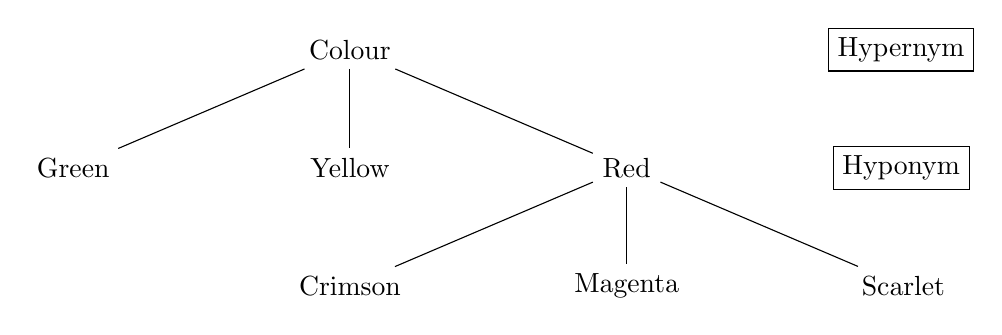
\begin{tikzpicture}[sibling distance=10em,
    every node/.style = {align=center}]]
    \node[draw] at (7,0) {Hypernym};
    \node[draw] at (7,-1.5) {Hyponym};
    \node {Colour}
    child { node {Green} }
    child { node {Yellow} }
    child { node {Red}
      child { node {Crimson} }
      child { node {Magenta} }
      child { node {Scarlet} }
    };
  \end{tikzpicture}
 \end{framed}
\caption{An example hypernym / hyponym hierarchy}
\label{fig:hyptree}
\end{figure}

Using different colours as an example, Figure \ref{fig:hyptree} shows the relationship of a hypernym parent and its hyponym child in a tree representation.

We can traverse a hypernym chain of parent nodes and determine a list of {\bf Semantic {\it Supersenses}}. Using top level word senses is the general methodology for creating a broad coverage supersense set of terms. WordNet has a closed set of top level hypernyms or supersenses which are used for broad coverage semantic word sense classification.

\begin{table}[!htbp]
  \centering
  \begin{tabular}{ |llll| }
    \hline
    n.Tops & n.act & n.animal & n.artefact\\
    n.attribute & n.body & n.cognition & n.communication\\
    n.event & n.feeling & n.food & n.group\\
    n.location & n.motive & n.object & n.person\\
    n.phenomenon & n.plant & n.possession & n.process\\
    n.quantity & n.relation & n.shape & n.state\\
    n.substance & n.time & v.body & v.change\\
    v.cognition & v.communication & v.competition & v.consumption\\
    v.contact & v.creation & v.emotion & v.motion\\
    v.perception & v.possession & v.social & v.stative\\
    v.weather & \  & \  & \ \\
    \hline
  \end{tabular}
  \caption{Noun and Verb Supersenses}
  \label{tab:wordnetsupersenses}
\end{table}

Table \ref{tab:wordnetsupersenses} shows the 41 top level Noun and Verb supersenses from WordNet. A generalised taxonomy of verbs and nouns is useful to broaden semantic scope. Using dictionaries for supervised learning by \cite{ciaramita2003supersense} introduced a framework of closed set supersenses which generalised well for unseen Named entities. 

The foundation for MWE and Supersense corpus was from hand-annotated Wikipedia articles performed by \cite{Schneider2012} which used a limited set of ``topics'' but relied heavily on expert knowledge by inexperienced annotators. These initial conclusions about broad supersense coverage motivates further broad class studies. Sequence tagging with an extended supersense set was interpreted as a type of Word Sense Disambiguation (WSD) task performed by \cite{Ciaramita2006} modifying the HMM model by \cite{collins2002discriminative}. Exploiting the POS tags syntactic context and the historical methodologies for sequence tagging proved to be an important baseline and ``offer a middle ground in granularity'' to generalise named entity classes and verbs\cite{Schneider2016}.

Supersenses in WordNet cover only nouns and verbs whereas adjectives do not have any type of hierarchical relationship. Additional studies extended taxonomic hierarchies to adjectives as performed by \cite{Tsvetkov2014} by using weakly supervised learning methods and crowdsourcing techniques. 

In addition, supersense tagged data corpora created using weakly supervised methodologies have been covered by \cite{Johannsen2014} and \cite{Owoputi2012} with the latter being provided \cite{dimsum16webdata} for use in the \dimsum shared task\cite{dimsum16web}. 

Supersenses by design are lexically assigned, coupled with a definition of MWEs, implies that Supersenses are just like other lexical items: Any single MWE can be assigned a Supersense.

\subsubsection{Word-Sense Disambiguation}

A dictionary entry, or ``citation form'' is referred to as a {\it lemma} in lexical semantics. A {\it lemma} can of course have many meanings referred to as {\it word senses} such as ``water'' meaning {\it liquid form of ${H_2}O$} or {\it to irrigate}. These {\it lemma} of multiple meanings are called {\it homonyms}. Being able to disambiguate a {\it word sense} in its context is referred to as {\bf Word-Sense Disambiguation}.
On the other hand, {\it Polysemy} is when the {\it word senses} are related in meaning. In addition to our previous example, ``water'' can also refer to a {\it body of water} such as ``the water is rough today'' when speaking about the ocean waves. These meanings of ``water'' could be said to be {\it Polysemous} since they both refer to {\it liquid ${H_2}O$} in some form, be it small or large. For readability, differing {\it word senses} are usually written with a superscript integer.

\begin{figure}[!htbp]
\centering
\begin{framed}
\begin{minipage}{.5\textwidth}
\centering
  \begin{tabular}{ | l | l | l |}
    \hline
    Sense & POS & Meaning\\
    \hline
    $Water^1$ & Noun & $H2O$\\
    $Water^2$ & Noun & body of water\\
    $Water^3$ & Verb & to irrigate\\
    \hline
  \end{tabular}
\end{minipage}\hfill
\begin{minipage}{.5\textwidth}
 \centering
 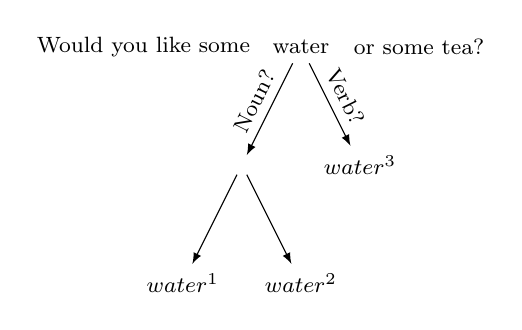
\begin{tikzpicture}
  [
    edge from parent/.style = {draw, -latex},
    every node/.style       = {font=\footnotesize},
    sloped
  ]
 \node at (-2,0) {Would you like some};
 \node at (1.5,0) {or some tea?};
 \node {water}
  child { node  {}
  child { node {$water^1$}}
  child { node {$water^2$}} edge from parent node [above] {Noun?} }
  child { node {$water^3$} edge from parent node [above] {Verb?} };
 \end{tikzpicture}
\end{minipage}
\end{framed}
\caption{An example WSD diagram}
\label{fig:decisionwsd}
\end{figure}

Figure \ref{fig:decisionwsd} shows a word sense table and decision tree representing the disambiguation choice by a computer system for an isolated word. Most modern systems do not make a singular choice in WSD tasks but rather use contextual or sequential information for word sense classification.

In addition to the traditional word disambiguation tasks, additional ``All-words'' WSD tasks have been proposed and studied. Instead of determining a specific word sense, systems learn all word senses and disambiguate in a larger phrasal context, such as sentence level\cite{Stetina1998}. Work by \cite{Ye2007} used Maximum Entropy models for preposition sense disambiguation which contrasted a type of BOW\footnote{Bag-Of-Words} model with surrounding POS tag information. Its results showed that ``collocation-based features'' were the most informative. Similar methodologies and results were done by \cite{Tratz2010} for nominals. 

\subsubsection{WSD and MWE}

Assigning supersenses to MWEs requires the ability to disambiguate their meaning from other potential meanings. This could occur due to syntactic ambiguity, inconsistent compositional parsing or competing context. While lexical ambiguity is more fine grained, both suffer from similar issues in Word Sense Disambiguation tasks. To disambiguate, we must have a sense of semantic relatedness, or semantic distance. Determining the most related sense should yield the obvious unambiguous conclusion for a given word. Semantic relatedness can be interpreted in statistical model, sequential, hierarchical or in graphs. Therefore distance can be determined given a model. There are many competing models but the initial heuristic for WSD systems is generally considered to be first-sense or predominant sense. A naive system which defaults to first-sense is used to determine the baseline capacity of a system. Considerable effort has been put into creating a reliable mechanism for evaluation such as methodologies developed by \cite{Lesk1986}. It hypothesised that observing textual context demonstrates relations which can be disambiguated using dictionaries.

In the Unsupervised All-words WSD using grammatical dependencies by \cite{Nastase2008}, a directed graph is used to determine word senses using the British National Corpus (BNC). Weights are placed on the edges and traversed to a root node, the best scoring path is used to disambiguate the word sense. The graph was created using a mixture of grammatical information for filtering interconnected nodes and semantic relations using the Word Sketch Engine\cite{Kilgarriff2014}. It also compared tie-breaking techniques for sense selection using PageRank and Lesk-based similarity. It showed that using grammatical constraints limit word-sense comparisons and help ``estimate selectional preference from an untagged corpus''\cite{Nastase2008}.

Most WSD tasks focus on the ability to disambiguate nouns and verbs. In the study by \cite{Hovy2010}, experiments of parameter choices for preposition disambiguation were analysed within its syntactic domain. Contextual dependencies of nouns, verbs and adjectives were observed in a fixed and selective window sizes to alleviate issues with conflation and sparsity. Prepositional phrases were labelled with one of seven classes and disambiguated using a Maximum Entropy model. Broader fixed window sizes showed higher accuracy, implying larger context has more semantic information. This idea is prevalent within the field and in line with the ``opaque mask'' formulation by \cite{weaver1955} stating ``if N is large enough one can unambiguously decide the meaning of the central word''. Interestingly, a selective dynamic window size based on syntactic heuristics performed better, outperforming \cite{OHara2009} which used only Fixed-window size.

A multilingual evaluation of techniques to automatically acquire MWEs from corpora was explored by \cite{Ramisch2012} which showed that the techniques with higher coverage of nominals had lower precision while higher precision techniques were inflexible. Alternative machine learning methodologies were suggested which could potentially play to the strengths for both approaches. 

A multilingual study used English resources to extend to foreign languages by detecting whether an MWE is a metaphor. \cite{Tsvetkov2013} used a methodology described as Common Semantic Features (CSF). It used a set of features in English to classify sentences as literal or metaphoric. The three features used included WordNet lexicographer file names, Vector Space Models to compute abstractness/concreteness and Named Entity types. Entities were recognised as SVO\footnote{Subject-Verb-Object} objects which used logistic regression to create a binary classifier. The algorithm was trained with English and evaluated on Russian. Interestingly, the difference in $F_1$ scores was within 2 percent for the Russian Model. Their claim was that semantic features are common as opposed to lexical features which are not, therefore the model could generalise well on Russian. The mixed feature based system created a rich and robust set of quantifiable concepts into a single algorithm but I have doubts that the model would generalise well on languages that have drastically different syntactic structures\footnote{Such as VSO languages like Gaelic or Tagalog}.

Many studies focus on a specific subset of MWE constructions, a broad coverage of entity constructions were covered by \cite{Schneider2014}. It used a rich and robust annotated social web corpus \cite{Schneider2014a} which is derived from the English Web Treebank \cite{bies2012english}. By using the structured perceptron with cost augmentation and features that recognise ``gappy'' structures, the task was one of the first supervised learning systems to identify heterogeneous MWEs. It has the ability to recognise strong and weak MWE constructions. Additional enhancements were introduced and implemented in the subsequent study \cite{Schneider2015} which added supersenses. This final study represents a state-of-the-art system for MWE recognition using supersenses \cite{Schneider2015}.
  
\subsubsection{Sequence labelling and Structured Prediction}

The \dimsum task can be interpreted as a sequence labelling task or a general structured prediction task. In the case of this dissertation, it is treated as such.

Sequence label prediction tasks such as POS tagging concentrate on sequential syntactic recognition in natural language processing. POS tagging systems are considered to have broad coverage for introduction of novel words within a contextual environment.

\begin{table}[!htbp]
  \centering
  \begin{tabular}{ lllllllll }
    The & man & in & the & black & shirt & trades & pokemon & cards\\
    \hline
    DT & NN & IN & DT & JJ & NN & VBZ & JJ & NNS\\
  \end{tabular}
  \caption{A POS Tagged Sentence}
  \label{tab:postagseq}
\end{table}

Table \ref{tab:postagseq} shows a POS tagged sequence\footnote{taken from the Stanford Natural Language Inference (SNLI) dataset \cite{bowman2015large}} which uses the Penn Treebank tagset\cite{Marcus1993}. The use of Hidden-Markov Models (HMM) for POS tagging\cite{Collins2002} has lead to reliable sequence tagging systems. If modelled properly, robust systems can tag unseen words, maintaining a minimum 85\% accuracy for the last decade \cite{brants2000tnt}. Creating methodologies for accurate POS tagged sentences laid the foundation for structured prediction labelling tasks.

\begin{figure}[H]
  \tikzset{font=\footnotesize}
  \centering
  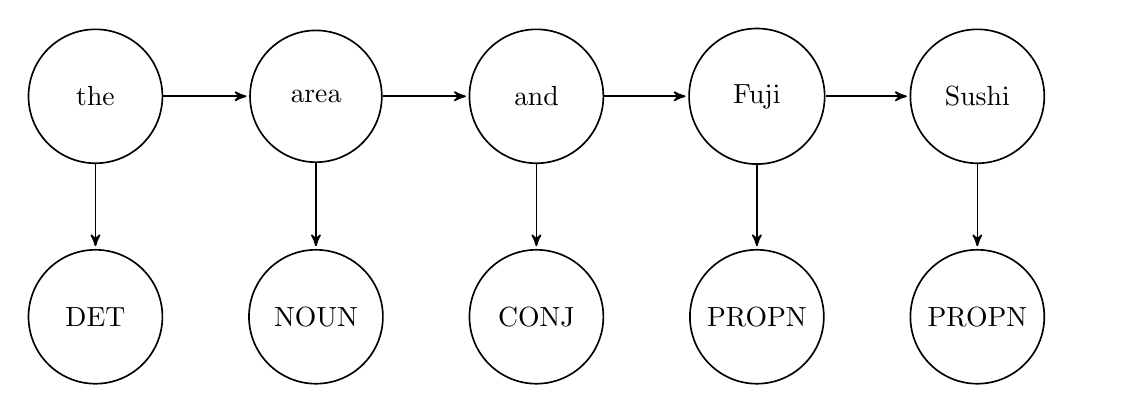
\begin{tikzpicture}[->,>=stealth',shorten >=1pt,auto,node distance=2.8cm,semithick,text width=1.4cm, align=center]
    \node[state] (A)              {the};
    \node[state] (B) [right of=A] {area};
    \node[state] (C) [right of=B] {and};
    \node[state] (D) [right of=C] {Fuji};
    \node[state] (E) [right of=D] {Sushi};
    \node[state] (F) [below of=A] {DET};
    \node[state] (G) [below of=B] {NOUN};
    \node[state] (H) [below of=C] {CONJ};
    \node[state] (I) [below of=D] {PROPN};
    \node[state] (J) [below of=E] {PROPN};

    \path
    (A) edge              node {} (B)
    (A) edge              node {} (F)
    (B) edge              node {} (C)
    (B) edge              node {} (G)
    (C) edge              node {} (D)
    (C) edge              node {} (H)
    (D) edge              node {} (E)
    (D) edge              node {} (I)
    (E) edge              node {} (J);
  \end{tikzpicture}
  \caption{Example HMM with POS tags from \dimsum data}
  \label{fig:hmmposdimsum}
\end{figure}

Named Entity Recognition (NER) was historically viewed as a type of Information Retrieval (IR) task but theoretically could be considered a specific subset of Multiword Expressions. Exploiting the tagging of nominals and augmenting structures with BIO-style\cite{Ramshaw1994} information leads to the ability to recognise {\bf B}eginning, {\bf I}nside and {\bf O}utside points in a Named Entities which is extended to be used in \dimsum for Multiword Expressions.

\begin{table}[!htbp]
\small
\begin{framed}
 \begin{tabular}{lllllllll}
  American & Airlines & , & a & unit & of & AMR & Corp. & ,\\ 
  NNP & NNPS & PUNC & DT & NN & IN & NNP & NNP & PUNC \\
  $B_{NP}$ & $I_{NP}$ & $O$ & $B_{NP}$ & $I_{NP}$ & $B_{PP}$ & $B_{NP}$ & $I_{NP}$ & $O$
 \end{tabular}\\ \ \\

 \begin{tabular}{llllllllll}
  immediately & matched & the & move & , & spokesman & Tim & Wagner & said & .\\
  RB & VBD & DT & NN & PUNC & NN & NNP & NNP & VBD & PUNC\\
  $B_{ADVP}$ & $B_{VP}$ & $B_{NP}$ & $I_{NP}$ & $O$ & $B_{NP}$ & $I_{NP}$ & $I_{NP}$ & $B_{VP}$ & $O$
 \end{tabular}
\end{framed}
 \caption{Sentence with BIO encoding and POS tags}
 \label{tab:biotagseq}
\end{table}

Table \ref{tab:biotagseq} shows an example POS tagged sentence with BIO encoding taken from an example in \cite{martin2000speech}. NER tasks can be therefore thought of as a subsumed precursor to Multiword Expression recognition tasks as NER sequences are contiguous while MWEs are syntactically flexible.

Work on ``exploiting syntactic forms'' by ``token classification of potential idioms'' \cite{Cook2007} intended to use features recognised in a narrow syntactic domain using Unsupervised learning to determine components as idiosyncratic. It proved to perform within a very narrow margin of error in comparison to its supervised counterparts (within 4\%) which were more concerned with a compositional approach. This type of syntactic narrow scope proved to be important in building informative generalisations. More modern studies show the relationship can be modelled simultaneously. Using Conditional Random Fields (CRF) by \cite{Constant2011} showed the ability to broaden the domain of NER to recognise noun and verb like idiomatic phrases.

Although syntactic information gives structure to sequences, a higher semantic scope is needed to broaden the context and generalise well. A overarching set of word senses are needed to encapsulate lexical and phrasal MWEs\footnote{Definitions of MWE types can be seen in section \ref{mwe}}. WordNet \cite{fellbaum1998wordnet} introduced a lexical database allowing generalisation into broad semantic supersenses.

Interpreting \dimsum as a structured prediction task we can broaden our model scope. Initial work using Conditional Random Fields (CRF) by \cite{lafferty2001conditional} and \cite{Collins2002} showed that sequence prediction using CRFs is possible and quite powerful, producing state-of-the-art results at the time.

As opposed to HMMs as seen in Figure \ref{fig:hmmposdimsum}, CRFs have the benefit of being able to use any input for label prediction. In Figure \ref{fig:crfwindowdimsum} we can see the current input \texttt{O} using a window size of 2 on either side for feature extraction.

\begin{figure}[H]
  \centering
  \tikzset{font=\footnotesize}
  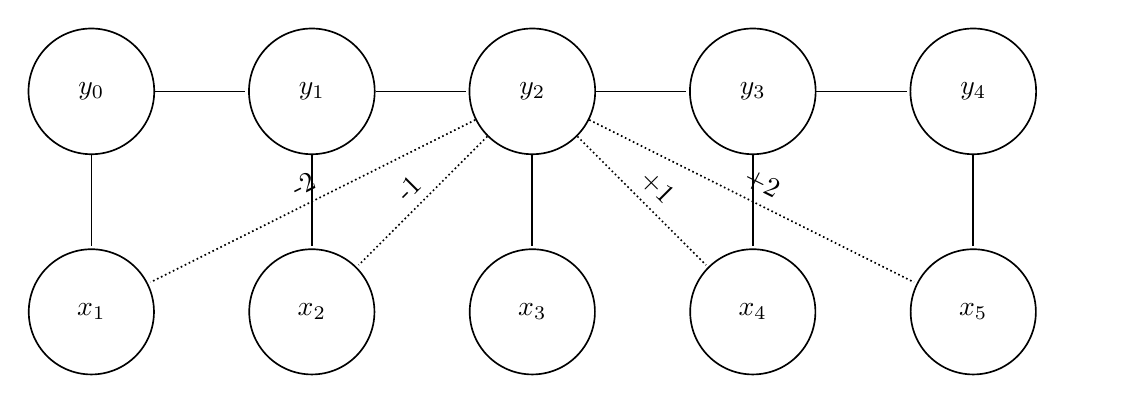
\begin{tikzpicture}[-,>=stealth',shorten >=1pt,auto,node distance=2.8cm,semithick,text width=1.3cm, align=center]
    \node[state] (A)              {$y_0$};
    \node[state] (B) [right of=A] {$y_1$};
    \node[state] (C) [right of=B] {$y_2$};
    \node[state] (D) [right of=C] {$y_3$};
    \node[state] (E) [right of=D] {$y_4$};
    \node[state] (F) [below of=A] {$x_1$};
    \node[state] (G) [below of=B] {$x_2$};
    \node[state] (H) [below of=C] {$x_3$};
    \node[state] (I) [below of=D] {$x_4$};
    \node[state] (J) [below of=E] {$x_5$};

    \path
    (A) edge              node {} (B)
    (A) edge              node {} (F)
    (B) edge              node {} (C)
    (B) edge              node {} (G)
    (C) edge              node {} (D)
    (C) edge              node {} (H)
    (D) edge              node {} (E)
    (D) edge              node {} (I)
    (E) edge              node {} (J);

    \path[draw, densely dotted]
    (C) edge              node [midway,above,sloped]{-2} (F)
    (C) edge              node [midway,above,sloped]{-1} (G)
    (C) edge              node [midway,above,sloped]{+1} (I)
    (C) edge              node [midway,above,sloped]{+2} (J);
  \end{tikzpicture}
  \caption{Example CRF showing $\pm$2 Window}
  \label{fig:crfwindowdimsum}
\end{figure}

Similar to the \dimsum task using Linear Chain CRFs a type of POS and MWE tagger by \cite{Constant2011} used different and smaller set of predefined senses. Moving towards the state of the art introduced the WordNet Supersenses while recognising syntactically flexible constrictions by \cite{Schneider2014}. The original \dimsum task publication mentions that two of the top three systems use CRFs for structured prediction. In fact, the baseline solution spoken of in Chapter \ref{chapter4} uses a CRF due to its proven track record in positive results. 

Many modern structured prediction systems are moving away from featured engineered systems with a preference towards a purely data driven model. Initial studies by \cite{collins2002discriminative} of a Structured perceptron prove the ability of multi-class labelling in the framework of POS tagging. By using a Neural Network approach, weights are optimised by learning from training data. Deep Neural Networks (DNN) have the ability to discriminate non-linearly allowing for non-binary labelling. \dimsum requires such capabilities are all label predictions are multi-class. Figure \ref{fig:nndiagram} shows a Neural Network with a Neuron and Activation layer\footnote{Original TikZ picture created by \cite{neuralnetdiagram}}.

%Neural Network
\begin{figure}[H]
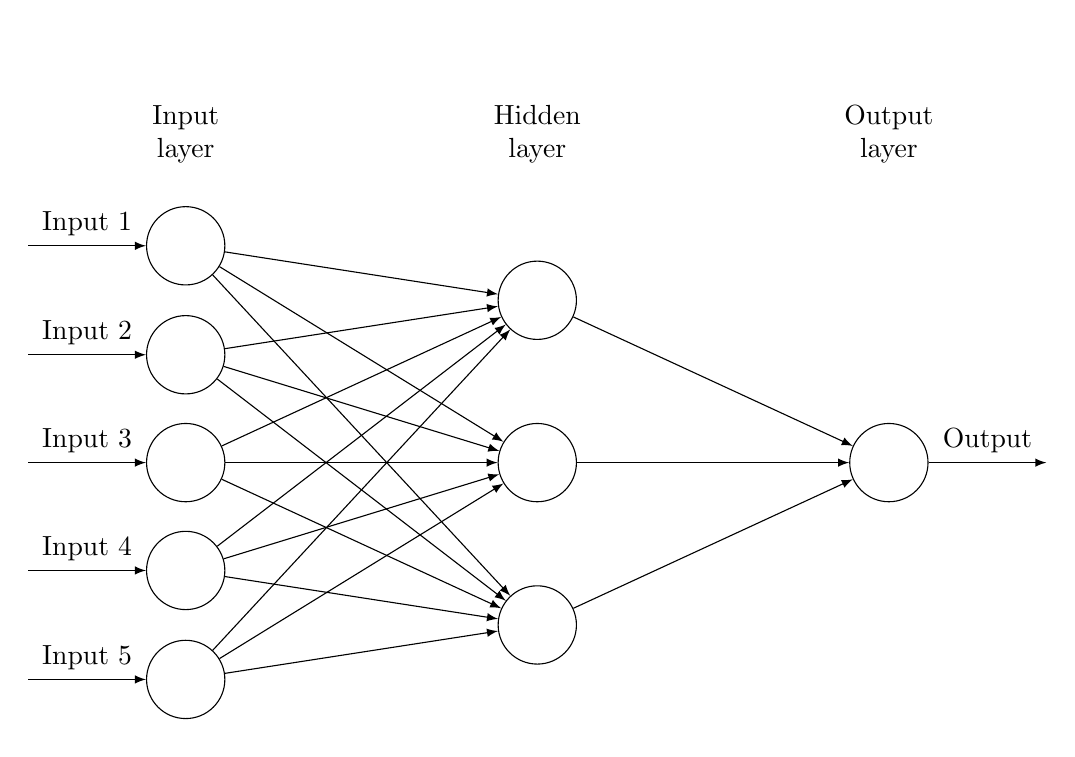
\begin{tikzpicture}[
plain/.style={
  draw=none,
  fill=none,
  },
net/.style={
  matrix of nodes,
  nodes={
    draw,
    circle,
    inner sep=10pt
    },
  nodes in empty cells,
  column sep=2cm,
  row sep=-9pt
  },
>=latex
]
\matrix[net] (mat)
{
|[plain]| \parbox{1.3cm}{\centering Input\\layer} & |[plain]| \parbox{1.3cm}{\centering Hidden\\layer} & |[plain]| \parbox{1.3cm}{\centering Output\\layer} \\
& |[plain]| \\
|[plain]| & \\
& |[plain]| \\
|[plain]| & |[plain]| \\
& & \\
|[plain]| & |[plain]| \\
& |[plain]| \\
|[plain]| & \\
& |[plain]| \\
};
\foreach \ai [count=\mi ]in {2,4,...,10}
  \draw[<-] (mat-\ai-1) -- node[above] {Input \mi} +(-2cm,0);
\foreach \ai in {2,4,...,10}
{\foreach \aii in {3,6,9}
  \draw[->] (mat-\ai-1) -- (mat-\aii-2);
}
\foreach \ai in {3,6,9}
  \draw[->] (mat-\ai-2) -- (mat-6-3);
\draw[->] (mat-6-3) -- node[above] {Output} +(2cm,0);
\end{tikzpicture}

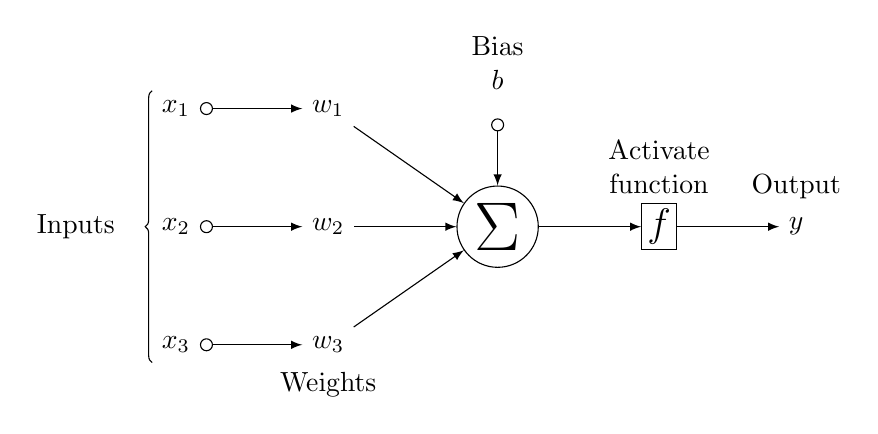
\begin{tikzpicture}[
init/.style={
  draw,
  circle,
  inner sep=2pt,
  font=\Huge,
  join = by -latex
},
squa/.style={
  draw,
  inner sep=2pt,
  font=\Large,
  join = by -latex
},
start chain=2,node distance=13mm
]
\node[on chain=2] 
  (x2) {$x_2$};
\node[on chain=2,join=by o-latex] 
  {$w_2$};
\node[on chain=2,init] (sigma) 
  {$\displaystyle\Sigma$};
\node[on chain=2,squa,label=above:{\parbox{2cm}{\centering Activate \\ function}}]   
  {$f$};
\node[on chain=2,label=above:Output,join=by -latex] 
  {$y$};
\begin{scope}[start chain=1]
\node[on chain=1] at (0,1.5cm) 
  (x1) {$x_1$};
\node[on chain=1,join=by o-latex] 
  (w1) {$w_1$};
\end{scope}
\begin{scope}[start chain=3]
\node[on chain=3] at (0,-1.5cm) 
  (x3) {$x_3$};
\node[on chain=3,label=below:Weights,join=by o-latex] 
  (w3) {$w_3$};
\end{scope}
\node[label=above:\parbox{2cm}{\centering Bias \\ $b$}] at (sigma|-w1) (b) {};

\draw[-latex] (w1) -- (sigma);
\draw[-latex] (w3) -- (sigma);
\draw[o-latex] (b) -- (sigma);

\draw[decorate,decoration={brace,mirror}] (x1.north west) -- node[left=10pt] {Inputs} (x3.south west);
\end{tikzpicture}
\caption{Diagram of a Neural Network and a Neuron}
\label{fig:nndiagram}
\end{figure}

One of the main issues with NNs is that long term dependencies are not captured well as weights are optimised over an entire training set. Long term dependencies are not ``remembered'' where as Recurrent Neural Networks (RNN) fix this issue. Long-Short Term Memory (LSTM) RNNs have additional weights and feedback mechanisms for capturing long term dependencies and ``remembering'' potentially useful information for discriminate labelling tasks. These feedback mechanisms can be thought of as a loop in a Neural Network or alternatively an unrolled sequence of RNNs as seen in Figure \ref{fig:rnnunrolled}\footnote{Figure taken from \cite{understandinglstmolah}}.

%Unrolled LSTM Image
\begin{figure}[H]
\centering
\includegraphics[width=0.8\textwidth]{images/RNN-unrolled.png}
\caption{Unrolled RNN}
\label{fig:rnnunrolled}
\end{figure}

Unlike a neural network's neuron, there are multiple non-linear activation functions which work together to ``remember'' details that would otherwise be forgotten in other DNNs as seen in Figure \ref{fig:lstmcell}\footnote{Figure taken from \cite{understandinglstmolah}}.

\begin{figure}[H]
\centering
\includegraphics[width=0.8\textwidth]{images/LSTM3-chain.png}
\caption{LSTM Chain cell}
\label{fig:lstmcell}
\end{figure}

Using LSTMs have proved very successful as seen in Machine Learning tasks such as \cite{Sutskever2014}. Additional usage of bidirectional features captures past and present memory of features inherent in training data as seen in \cite{Graves2005} for phoneme classification. Using both concepts lead to Bidirectional LSTM usage with a CRF layer as seen in \cite{Lample2016} which showed state of the art results in a completely data driven approach to NER. 

\section{Discussion}
A well adapted system to perform the \dimsum task will require the ability to assign useful semantic tags to lexical items and heterogeneous MWEs. This entails the ability to recognise weak and strong MWE constructions with ``gappy'' structures. Statistics drawn from \cite{Schneider2014} show that around 75\% of constructions are strong, i.e. {\bf Fixed Expressions} or {\bf Institutionalised Phrases}, but the additional 25\% are weak being {\bf Semi-Fixed Expressions} or {\bf Syntactically-Flexible Expressions}. Choosing to ignore these ``gappy'' constructions shows ``loss in performance''\cite{Schneider2014} which is to be expected. As seen previously, \cite{Ramisch2012} confirms that coverage of a specific lexical category can be modelled to have high coverage but low overall performance\footnote{``Cover most of the nominals... having lower precision'' \cite{Ramisch2012}}. 

It is a pervasive belief that semantic senses are common across languages whereas lexical features are not. For a robust and generalised system, a scope which encompasses supersenses on lexical items should be used. Ideally, being portable and scalable are equally important which implies elegant algorithms and availability of labelled data or more intricate models with unlabelled data. At this point, state-of-the art systems rely on structural data. 
Therefore, the initial baseline for \dimsum should include these features that capture structure and generalise meaning well. This should include multi-category MWE recognition and supersense tagging. 

Since there are many research topics that lead to positive results using CRFs, initial baseline construction will follow suit. In addition, a network architecture approach using LSTMs will be created in addition. More details on design can be read about in Chapter \ref{chapter4}.


\chapter{Requirements and Analysis}\label{chapter3}
% This should state, in a more detailed way, the objectives of the project by requirement and the analysis should break the problem down into manageable steps. There may be more than one suitable approach; the analysis may cover more of the area than is finally implemented. Testing and evaluation should be given due consideration. It is important that you state how you will evaluate your work. For a design project it is appropriate to consider testing at the same time as specification.

This chapter will speak about solution requirements, objectives and data. In the first section, a basic idea of the aim of the solution will be discussed. The requirements will follow giving more details about the data and predictive requirements for the task. The analysis sections will speak about statistics on data and draw some broad  conclusions about what to expect, while the final section will speak about how to approach creating a solution in manageable, modular steps.

\section{Aims and Objectives}

The main goal is to create a system which will predict MWE and Supersense tags as outlined in the original \dimsum task \cite{Schneider2016}. The solution should include a sensible baseline and a system which outperforms the baseline. A sensible solution can be quantified as a system which performs within the results for the original task with an F1-Score of 27-57\%. Therefore the requirements section will speak about the baseline system and the final system within this framework. 

\section{Requirements}

The original SemEval Task 10 \dimsum defines requirements for the data and output of the system. Certain aspects of the requirements are previously defined and will be mentioned briefly here. Additional requirements were self-imposed due to constraints or deliberate choices. All will be discussed in the following sections.

\subsection{Data}
The data requirements are fairly well defined in the \dimsum task. Additional information about the data and its usage can be seen in the appendix \ref{appendixdata}. Sentences are provided in a CoNLL style file separated by newlines which contain nine columns as seen in Figure \ref{fig:dimsumcolumns}.

\begin{figure}[H]
\centering
\begin{framed}
  \centering
  \begin{ttfamily}
    \begin{enumerate}
      \setlength{\itemsep}{0pt}
      \setlength{\parskip}{0pt}
    \item token offset
    \item word
    \item lowercase lemma
    \item POS
    \item MWE tag
    \item offset of parent token
    \item strength level encoded (unused)
    \item supersense label, if applicable
    \item sentence ID
    \end{enumerate}
  \end{ttfamily}
\end{framed}
\caption{Sentence columns for \dimsum data}
\label{fig:dimsumcolumns}
\end{figure}

There are no constraints on types of systems such as rule based vs. data driven methodologies therefore any column can be used for training. The final results must predict labels in columns 5 and 8. Column number 6 must also be filled in but is deterministically defined by the prediction of the MWE labels in column 5. The labelled training files provided for the \dimsum task in \cite{dimsum16webdata} contain sentences with the columns identical to Figure \ref{fig:dimsumcolumns} with ``\texttt{blind}'' testing file counterparts which contain blank or obfuscated labels. An example sentence can be seen in Figure \ref{tab:dimsumsentence} below, taken from \texttt{dimsum16.train}, the main training data file.

\begin{table}[!htbp]
\small
\begin{framed}
  \centering
  \begin{ttfamily}
  \begin{tabular}{lllllllll}
    1 & So & so & ADV & O & 0 &  &  & ewtb.r.328828.6\\
    2 & what & what & PRON & O & 0 &  &  & ewtb.r.328828.6\\
    3 & was & be & VERB & O & 0 &  & v.stative & ewtb.r.328828.6\\
    4 & the & the & DET & B & 0 &  & n.communication & ewtb.r.328828.6\\
    5 & point & point & NOUN & I & 4 &  &  & ewtb.r.328828.6\\
    6 & of & of & ADP & O & 0 &  &  & ewtb.r.328828.6\\
    7 & the & the & DET & O & 0 &  &  & ewtb.r.328828.6\\
    8 & appointment & appointment & NOUN & O & 0 &  & n.event & ewtb.r.328828.6\\
    9 & !?! & !?! & PUNCT & O & 0 &  &  & ewtb.r.328828.6\\
  \end{tabular}
  \end{ttfamily}
  \caption{Example sentence in \dimsum training file dimsum16.train}
  \label{tab:dimsumsentence}
\end{framed}
\end{table}

All predictions must be made in the same order as the \texttt{blind} test file with the appropriate columns filled in (5,6,8). Column 9 is just for cross referencing where the sentence was retrieved from by using an unambiguous ID. In the \texttt{blind} test files it is usually filled in with an obfuscated form of the sentence ID. It is not needed for the final prediction and can be left untouched. 

Any pre or post-processing is acceptable just as long as the first 4 columns can be recreated or inferred from the original test sentence.

The data given for the \dimsum task contains an evaluation script called \texttt{dimsumeval.py}. In order to compare the results in a meaningful way, all evaluation must use this script in conjunction with the data files provided for the task. This will be spoken about in more detail in the analysis section that follows.

Any additional details on how the data was obtained and annotated can be viewed in the paper \cite{Schneider2015}.

Finally, any solution should generalise to unseen data, using labels defined in the dataset itself. 

\subsection{Prediction}
This section speaks about the requirements for the prediction of the MWEs and supersenses as well as data sparsity related issues.

\subsubsection{Multiword Expressions}
MWEs can take multiple forms in the \dimsum data. They are categorised as contiguous or gappy constructions, essentially forms of weak and strong MWEs. Due to this, the data uses a modified \texttt{BIO} style annotation with additional lowercase forms to capture ``gappy'' constructions, making possible MWE tags \texttt{BbIiOo}. The tag scheme follows the predictable scheme of {\bf B}eginning, {\bf I}nside, {\bf O}utside with the corresponding lowercase forms to capture the embedded constructions in gappy MWEs. In complete contrast to Named Entity Recognition tasks, gappy constructions {\it can} exist within the \dimsum MWE labels, which capture a wider degree of flexibility inherent in natural language. This makes the task more complex but more realistic.

\begin{table}[!htbp]
\small
\begin{framed}
  \centering
  \begin{ttfamily}
  \begin{tabular}{llllllllllll}
    I & have & a & bit & of & experience & watching & the & usual & assembly & line \\
    PRON & VERB & DET & NOUN & ADP & NOUN & VERB & DET & ADJ & NOUN & NOUN \\
    O & B & b & i & o & I & O & O & O & B & I \\
    \ & \ & \multicolumn{3}{c}{$\underbrace{\hspace{2.5cm}}$} & & & & & & \\ 
    \ & \ & \multicolumn{3}{c}{Embedded MWE} & & & & & & \\ 
    \ & \multicolumn{5}{l}{$\underbrace{\hspace{5.5cm}}$} & & & & & \\ 
    \ & \multicolumn{5}{c}{Gappy MWE} & & & & & \\ 
  \end{tabular}
  \end{ttfamily}
  \caption{Example ``gappy'' construction in training data}
  \label{tab:gappysentence}
\end{framed}
\end{table}

The difficulty in predicting such constructions requires a recognition of contiguous {\it and} gappy constructions. This is how the \dimsum task is unique from other Named Entity Recognition systems. Creating a generalisable solution is important for capturing these differences. 

\subsubsection{Supersenses}

All available top level Supersenses are represented in the training data as can be seen in \ref{tab:wordnetsupersenses}. There are 26 \texttt{NOUN} heads and 15 \texttt{VERB} heads, this means that there is a possible 41 supersense tags to be considered. The prediction of supersenses is not limited to MWEs and can be assigned to any single word which might carry semantic content. Assigning a correct supersense tag therefore depends on both cases. If a supersense is assigned to a word, it will appear in it's appropriate column in the training data for that specific word, whereas a MWE that contains a supersense tag must be assigned to it's head which are the tags \texttt{Bb} respectively. 

For example, as seen in Figure \ref{tab:dimsumsentence}, line 3 has the tag \texttt{v.stative} assigned to the word \texttt{was}, whereas line 4 has the tag \texttt{n.communication} assigned to it with the following line 5 being empty as the semantic supersense has already been assigned to the previous token. 

\begin{table}[!htbp]
\small
\begin{framed}
  \centering
  \begin{ttfamily}
    \begin{minipage}{.5\textwidth}
      \centering
      \begin{tabular}{ll}
        \multicolumn{2}{c}{Correctly Assigned Supersense}\\
        \hline
        Sihuan  & Pharmaceutical \\
        PROPN   & NOUN \\
        B       & I \\
        n.group &\\
      \end{tabular}
    \end{minipage}\hfill
    \begin{minipage}{.5\textwidth}
      \centering
      \begin{tabular}{ll}
        \multicolumn{2}{c}{Incorrectly Assigned Supersense}\\
        \hline
        Sihuan  & Pharmaceutical \\
        PROPN   & NOUN \\
        B       & I \\
        \ & n.group\\
      \end{tabular}
    \end{minipage}\hfill
  \end{ttfamily}
  \caption{Example correct/incorrect MWE supersense tagging}
  \label{tab:supersensetagging}
\end{framed}
\end{table}

As seen in the previous example in Table \ref{tab:supersensetagging}, the first example has only one assigned supersense to the head with the \texttt{B} MWE tag. The incorrect example shows the supersense assigned to the \texttt{I} MWE tag which does not follow the constraints.

These constraints must be maintained or the semantic supersense tags predicted will be considered incorrect and evaluation will not work correctly. That being said, all solutions must stick to this constraint and assign a single supersense per word or per MWE head for all words contained within the MWE.

The idea for these constraints is to assigned semantic information to single semantic units. Since MWEs are considered to be a single semantic unit, irrespective of their construction, only a single semantic sense should be assigned. 

A solution to the \dimsum task must take these constraints into account when predicting supersenses.

\section{Analysis}
In this section, an analysis of the data and project will be explained, with an attempt to clarify data and draw initial conclusions. 

Initially, looking at some statistics related to the training data was the first was step taken to give us insight on task. The following is stated in the \texttt{TAGSET.md} file in the \dimsum data. 

\begin{table}[H]
\centering
\begin{tabular}{|cccccc|}
\hline
      & \multicolumn{2}{c}{Not inside gap} & \multicolumn{2}{c}{Inside gap} & \\
\hline
      & Count & Token & Count & Token & \\
\hline
\hline
      & 63264 & O & 675 & o & \\
      &  4208 & B & 24  & b & \\ 
      &  5623 & I & 32  & i & \\
\hline
\hline
      &       &   &     &   & All tokens\\
\hline
Total & 73095 &   & 731 &   & 73826\\
\hline
\end{tabular}
\caption{Token-level MWE-positional flags with frequency counts}
\label{tab:mwetokencounts}
\end{table}

Supersense count statistics shed light on the frequency of noun or verb types as seen in Table \ref{tab:ssnvcounts}.

\begin{table}[H]
\centering
\begin{tabular}{cc}
noun  & verb\\
\hline
12591 & 9863\\
\end{tabular}
\caption{Supersense frequency counts in \dimsum training data}
\label{tab:ssnvcounts}
\end{table}

Finally, the top counts of each supersense are demonstrative relative clues for semantic nature of MWEs.

\begin{table}[H]
\centering
\begin{tabular}{lcc}
n.person & v.stative\\
\hline
1867     & 3357\\
\end{tabular}
\label{tab:topssnvcounts}
\caption{Top supersense frequency counts per category}
\end{table}

From the statistics in the original \texttt{TAGSET.md} file we can state the following.

{\bf The majority of:}
\begin{enumerate}
  \setlength{\itemsep}{0pt}
  \setlength{\parskip}{0pt}
\item MWE Tokens are \texttt{O}
\item MWEs are not gappy
\item Supersenses are noun types
\item Noun supersenses are n.person
\item Verb supersenses are v.stative
\end{enumerate}

Since the majority of MWE tokens are \texttt{O}, we know that the majority of words are {\bf O}utside an MWE. Also, most MWEs are strong or continuous as only a small minority are the gap internal counterpart labels. This inherently means most MWEs are not weak, so our system should at least be able to recognise continuous MWEs well as well at use the outside tag in a correct way. It could potentially use it for unseen data considering it to be the safest conclusion to make as it is the most common label on a per token basis. This is in fact the case as described in Chapter \ref{chapter4}, the default label is \texttt{O} for unseen data.

An additional script was written to read the data files provided with the task which sheds additional light on the relationship of supersenses for MWEs.

\begin{figure}[H]
\centering
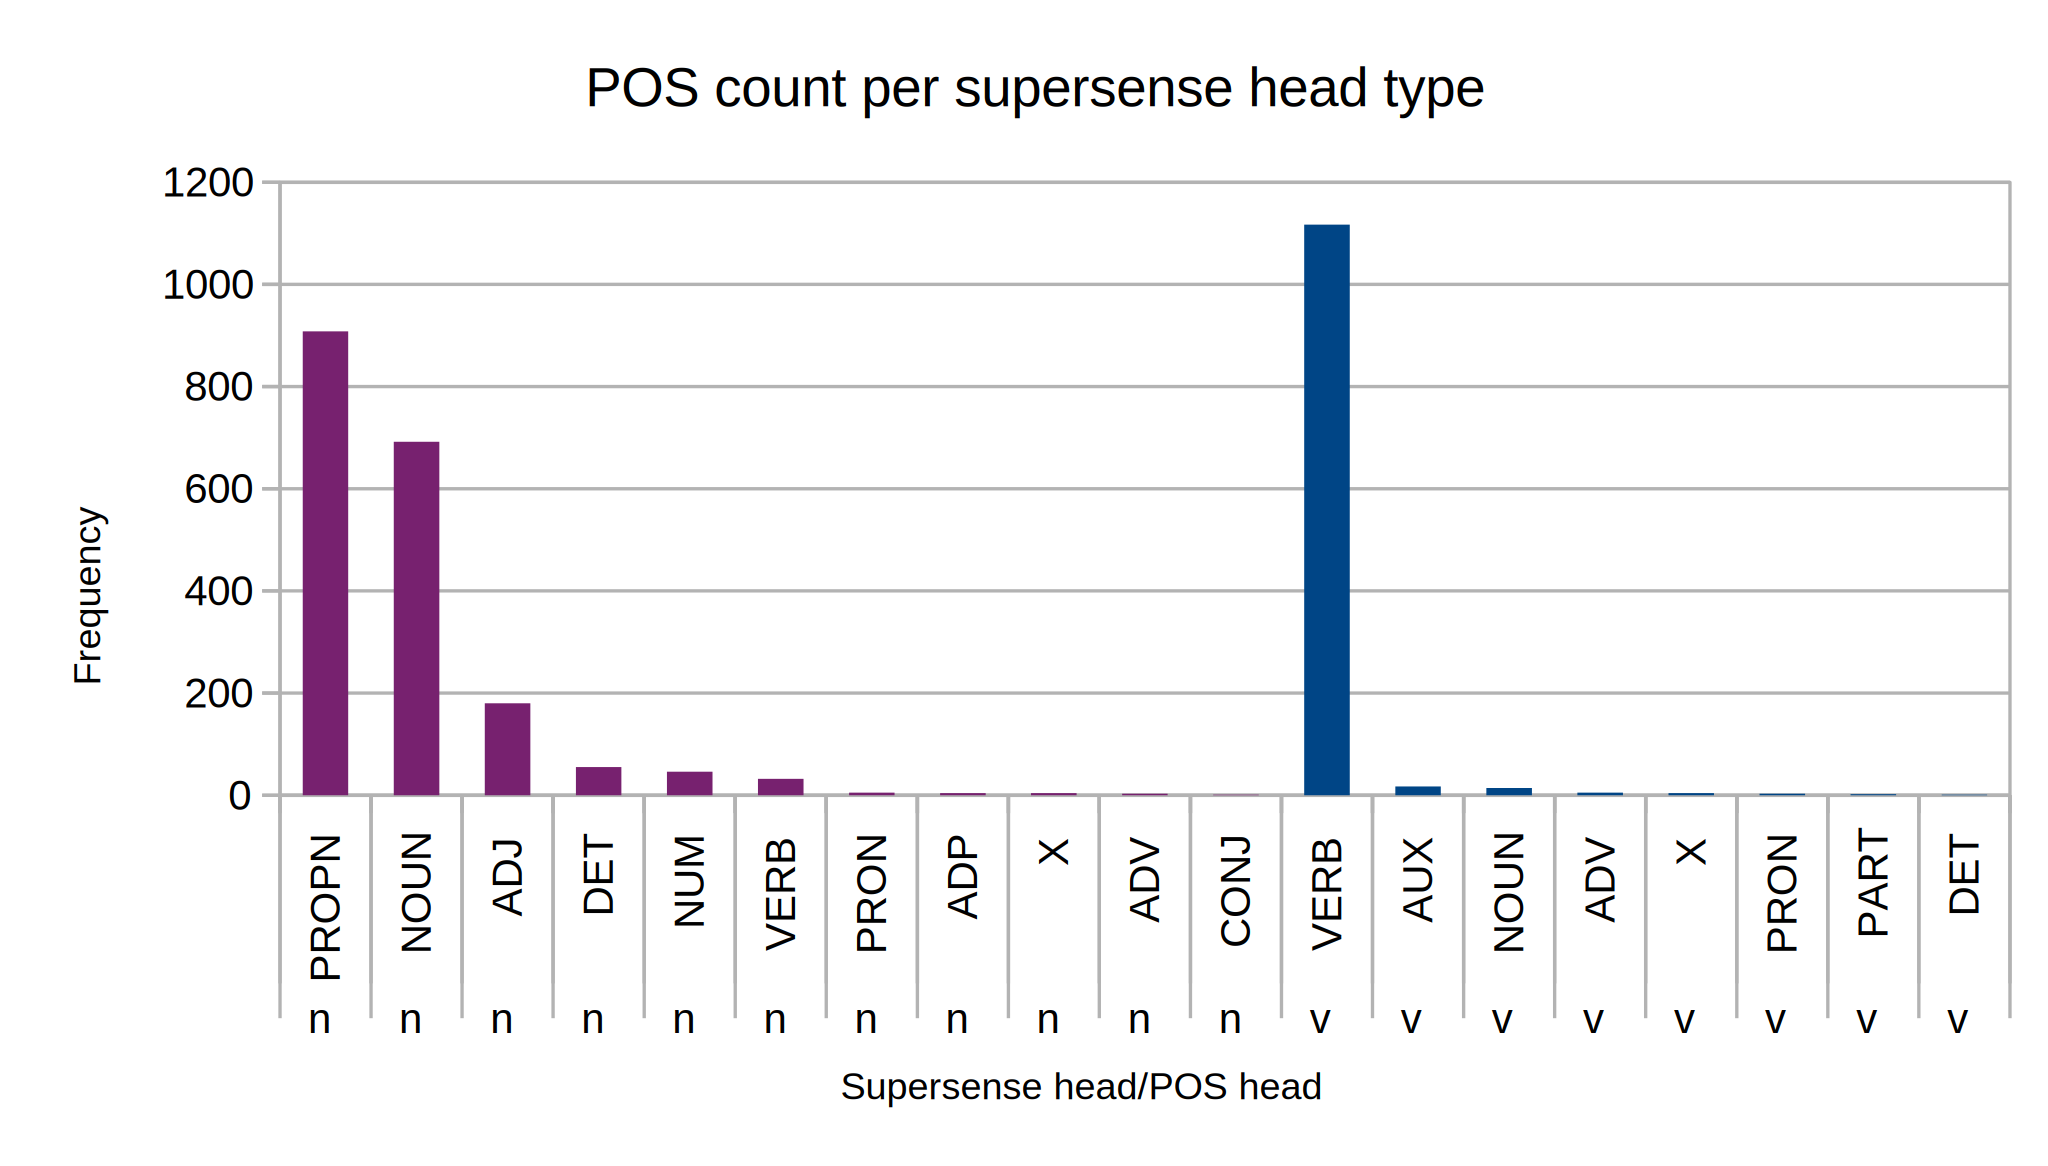
\includegraphics[width=0.8\textwidth]{images/pos_ss_freq.png}
\caption{POS frequency count per Supersense Head type}
\label{fig:posfreqperss}
\end{figure}

Figure \ref{fig:posfreqperss} shows the quantity of times a POS tag is seen for a given super sense head type (either n. or v.). This shows that the majority of times a noun supersense is tagged, its corresponding head is a proper noun. This in conjunction with the fact that most supersenses are tagged \texttt{n.person} would lead us to believe many noun headed supersenses are in fact named entities. Almost all verb headed supersenses have a POS tag of VERB which is not so informative. What is informative is the lower counts which show that many verb headed supersenses do not have a POS tag of VERB. 

These statistics give us information about what single types of supersense or MWE tags are occurring in the data but are uninformative in regards to context. Contextual clues will give us the information to create a robust solution. 

\section{Modularity and Procedure}

This final section will attempt to use the previous information in this chapter to outline a meaningful approach to modularising data and results into different stages. These stages will help draw conclusions about the systems, their predictive capacity and robustness of solution.

\subsection{Baseline system}
The baseline system should be a full solution to the task which uses a sensible albeit simple approach. The original paper \cite{Schneider2016} defined multiple systems and the highest scoring system used Conditional Random Fields. Therefore a CRF will be used to create the baseline system. The baseline should give information about a minimum F1-Score to achieve while simultaneously giving details about which features are more useful for creating a robust solution. 

The following steps should occur when creating a baseline:
\begin{enumerate}
  \setlength{\itemsep}{0pt}
  \setlength{\parskip}{0pt}
\item Create basic CRF solution
\item Vary features of initial solution
\item Vary window of initial solution
\item Use highest scoring baseline to draw conclusions on data
\item Use conclusions to create robust final system
\end{enumerate}

The baseline therefore serves two purposes, to create a solution which performs within the original task's framework, and helps determine meaningful information about the data to help design a more robust final solution. 

Many of the systems followed the most restrictive guidelines when using data, which was called the ``Supervised closed'' data condition which allows only the use of the training data provided without any outside data sources. The baseline solution will be within this data condition as a further limitation to set a sensible lower limit. 

\subsection{Final system}

The final system should take the connections drawn from the baseline into account and try to exploit its strengths. Since the baseline uses the most restrictive data condition for the task, the final system should use the most unrestrictive. Using the most restrictive data condition for the baseline will potentially restrict scope and ability of training, leading to less general and poorer results, which should create a more meaningful lower limit for the F1-Score. Using the least restrictive data condition should generalise better and create a more robust solution as more data in data driven classification systems commonly increase performance. 

At this time a Recurrent Neural Network design is suggested and therefore will be the initial choice for the final system. The basic procedure for creating the solution should be as follows. 

\begin{enumerate}
  \setlength{\itemsep}{0pt}
  \setlength{\parskip}{0pt}
\item Review data from CRF baseline
\item Use CRF baseline data analysis for RNN
\item Create basic RNN solution using ``Supervised closed'' data condition.
\item Create robust ``open'' data condition RNN solution
\item Evaluate all systems and compare
\end{enumerate}

In order to compare all solutions effectively, the provided \texttt{dimsumeval.py} will be used for all evaluation. It will allow for cross comparison between systems and help identify possible relationships between data, parameters and behaviours of predictions.

\chapter{Design}\label{chapter4}

The design chapter will outline the design choices and their justifications for the baseline and final system. The algorithms for the baseline systems will be discussed and used to help justify further design for the final system. Finally, parameters and details about the adapted Bi-LSTM-CRF design will be discussed in greater detail.

\section{CRF Baseline}

The starting point for design of a CRF system is simply a justification for model use. A CRF is flexible and can capture long distance features since it is not bound on inputs for a given label. This gives it a unique advantage in generalising labels given a rich feature set. As mentioned in the previous chapter, the CRF performed better over other designs. Due to this and my previously mentioned motivations, it seems the obvious choice for a starting point.

\begin{figure}[H]
  \centering
  \tikzset{font=\footnotesize}
  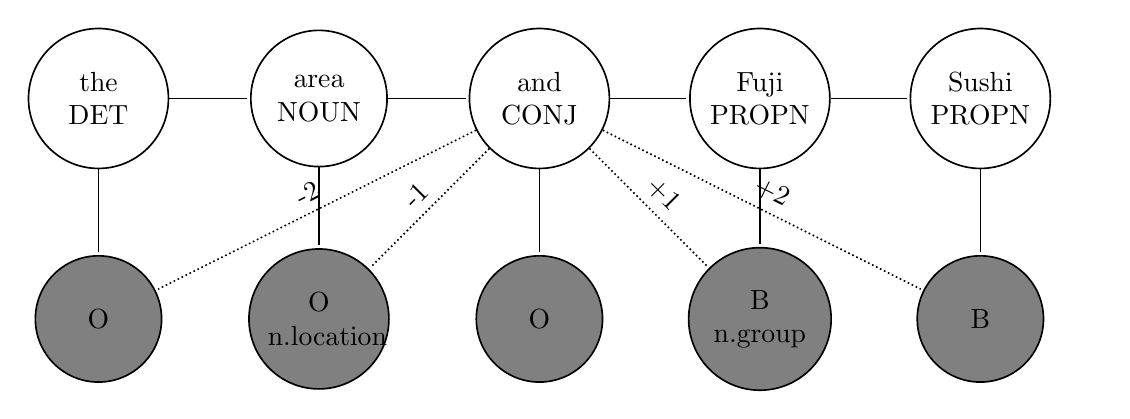
\begin{tikzpicture}[-,>=stealth',shorten >=1pt,auto,node distance=2.8cm,semithick,text width=1.3cm, align=center]
    \node[state] (A)              {the\\ DET};
    \node[state] (B) [right of=A] {area\\ NOUN };
    \node[state] (C) [right of=B] {and\\ CONJ };
    \node[state] (D) [right of=C] {Fuji\\ PROPN};
    \node[state] (E) [right of=D] {Sushi\\ PROPN};
    \node[state,fill=gray] (F) [below of=A] {O};
    \node[state,fill=gray] (G) [below of=B] {O\\ n.location};
    \node[state,fill=gray] (H) [below of=C] {O};
    \node[state,fill=gray] (I) [below of=D] {B\\ n.group};
    \node[state,fill=gray] (J) [below of=E] {B};

    \path
    (A) edge              node {} (B)
    (A) edge              node {} (F)
    (B) edge              node {} (C)
    (B) edge              node {} (G)
    (C) edge              node {} (D)
    (C) edge              node {} (H)
    (D) edge              node {} (E)
    (D) edge              node {} (I)
    (E) edge              node {} (J);

    \path[draw, densely dotted]
    (C) edge              node [midway,above,sloped]{-2} (F)
    (C) edge              node [midway,above,sloped]{-1} (G)
    (C) edge              node [midway,above,sloped]{+1} (I)
    (C) edge              node [midway,above,sloped]{+2} (J);
  \end{tikzpicture}
  \caption{Example Baseline CRF showing $\pm$2 Word Window with from \dimsum data}
  \label{fig:crfwindowgraydimsum}
\end{figure}

\subsection{Algorithms}
There are three CRF baselines created for varying purposes. The choices for the different approaches will be mentioned here and expanded upon in the following chapters.

The initial baseline used two CRFs to predict the MWE tag sequence and the Supersense tag sequence. The Second CRF uses the MWE sequence prediction from the first CRF as features. 

\subsubsection{Baseline 1 Algorithm:}
\begin{mdframed}[
    linewidth=0pt,
    roundcorner=4pt,
    backgroundcolor=gray!15,
    userdefinedwidth=\textwidth,
]
\begin{enumerate}
\tiny
  \setlength{\itemsep}{0pt}
  \setlength{\parskip}{0pt}
\item Extract features from training data with $\pm 2$ word context (Lemma+POS Tags)
\item Train MWE CRF to predict MWE Tags using features in (1)
\item Predict MWE tag sequences using CRF in (2)
\item Extract features from training data and predicted MWE tags with $\pm 2$ word context (Lemma+POS Tags+MWE tags)
\item Train Supersense CRF to predict Supersense Tags using features in (4)
\item Predict Supersense tag sequences using testing data and predictions from (3)
\item Systematically create parent offset sequences for MWE sequences
\item Combine MWE and Supersense predictions in (6) with parent offset sequences in (7) for final predictions
\end{enumerate}
\end{mdframed}

Viewing the algorithm for baseline 1 in an alternative way, as seen in Figure \ref{fig:crfbaseline1}, we can see that the prediction of MWE tags in the first CRF layer is used as features for the input of the second CRF layer. Their combined MWE and supersense predictions are used for the final prediction output for baseline number 1.

\begin{figure}[H]
  \centering
  \tikzset{font=\footnotesize}
  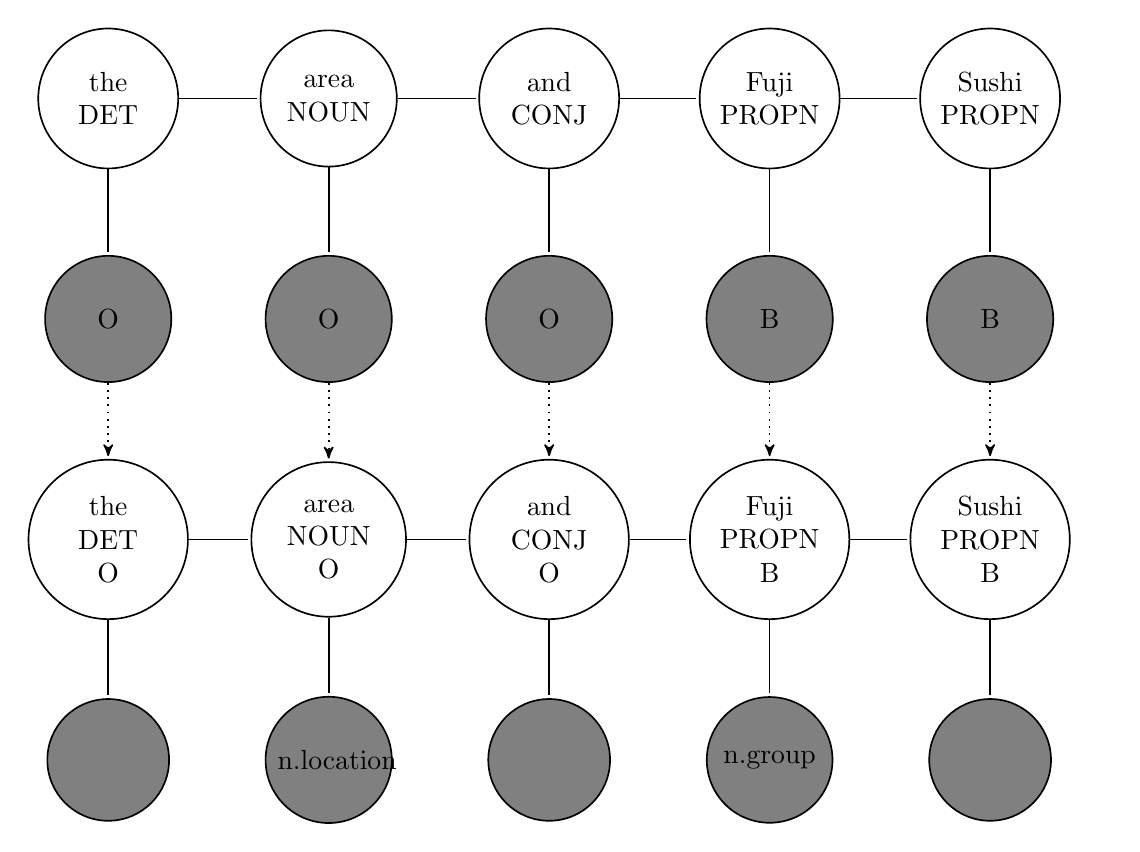
\begin{tikzpicture}[-,>=stealth',shorten >=1pt,auto,node distance=2.8cm,semithick,text width=1.3cm, align=center]
    \node[state] (A)              {the\\ DET};
    \node[state] (B) [right of=A] {area\\ NOUN };
    \node[state] (C) [right of=B] {and\\ CONJ };
    \node[state] (D) [right of=C] {Fuji\\ PROPN};
    \node[state] (E) [right of=D] {Sushi\\ PROPN};
    \node[state,fill=gray] (F) [below of=A] {O};
    \node[state,fill=gray] (G) [below of=B] {O};
    \node[state,fill=gray] (H) [below of=C] {O};
    \node[state,fill=gray] (I) [below of=D] {B};
    \node[state,fill=gray] (J) [below of=E] {B};

    \node[state] (K) [below of=F]  {the\\ DET\\ O};
    \node[state] (L) [below of=G] {area\\ NOUN\\ O};
    \node[state] (M) [below of=H] {and\\ CONJ\\ O};
    \node[state] (N) [below of=I] {Fuji\\ PROPN\\ B};
    \node[state] (O) [below of=J] {Sushi\\ PROPN\\ B};
    \node[state,fill=gray] (P) [below of=K] {};
    \node[state,fill=gray] (Q) [below of=L] {n.location};
    \node[state,fill=gray] (R) [below of=M] {};
    \node[state,fill=gray] (S) [below of=N] {n.group};
    \node[state,fill=gray] (T) [below of=O] {};
    % paths connecting inital CRF
    \path
    (A) edge              node {} (B)
    (A) edge              node {} (F)
    (B) edge              node {} (C)
    (B) edge              node {} (G)
    (C) edge              node {} (D)
    (C) edge              node {} (H)
    (D) edge              node {} (E)
    (D) edge              node {} (I)
    (E) edge              node {} (J);
    % paths connecting predictions in inital CRF
    \path[->, draw, dotted]
    (F) edge              node {} (K)
    (G) edge              node {} (L)
    (H) edge              node {} (M)
    (I) edge              node {} (N)
    (J) edge              node {} (O);
    % paths for output CRF
    \path
    (K) edge              node {} (L)
    (K) edge              node {} (P)
    (L) edge              node {} (M)
    (L) edge              node {} (Q)
    (M) edge              node {} (N)
    (M) edge              node {} (R)
    (N) edge              node {} (O)
    (N) edge              node {} (S)
    (O) edge              node {} (T);

  \end{tikzpicture}
  \caption{CRF Baseline 1}
  \label{fig:crfbaseline1}
\end{figure}

\subsubsection{Baseline 2 Algorithm:}
The second baseline is almost identical to the first except is uses the same features for both sequence predictions allowing for comparisons of advantages and disadvantages of features in a quantifiable manner.

\begin{mdframed}[
    linewidth=0pt,
    roundcorner=4pt,
    backgroundcolor=gray!15,
    userdefinedwidth=\textwidth,
]
\begin{enumerate}
\tiny
  \setlength{\itemsep}{0pt}
  \setlength{\parskip}{0pt}
\item Extract features from training data with $\pm 2$ word context (Lemma+POS Tags)
\item Train MWE CRF to predict MWE Tags using features in (1)
\item Predict MWE tag sequences using CRF in (2)
\item Extract features from training data and predicted MWE tags with $\pm 2$ word context (Lemma+POS Tags)
\item Train Supersense CRF to predict Supersense Tags using features in (4)
\item Predict Supersense tag sequences using testing data and predictions from (3)
\item Systematically create parent offset sequences for MWE sequences
\item Combine MWE and Supersense predictions in (6) with parent offset sequences in (7) for final predictions
\end{enumerate}
\end{mdframed}

Viewing the algorithm for baseline 2 in an alternative way, as seen in Figure \ref{fig:crfbaseline2}, we can see that the prediction of MWE tags in the first CRF layer is done independently of the prediction of Supersenses in the second CRF layer. The independently predicted MWE and Supersense results are then combined for the final prediction output for baseline number 2.

\begin{figure}[H]
  \centering
  \tikzset{font=\footnotesize}
  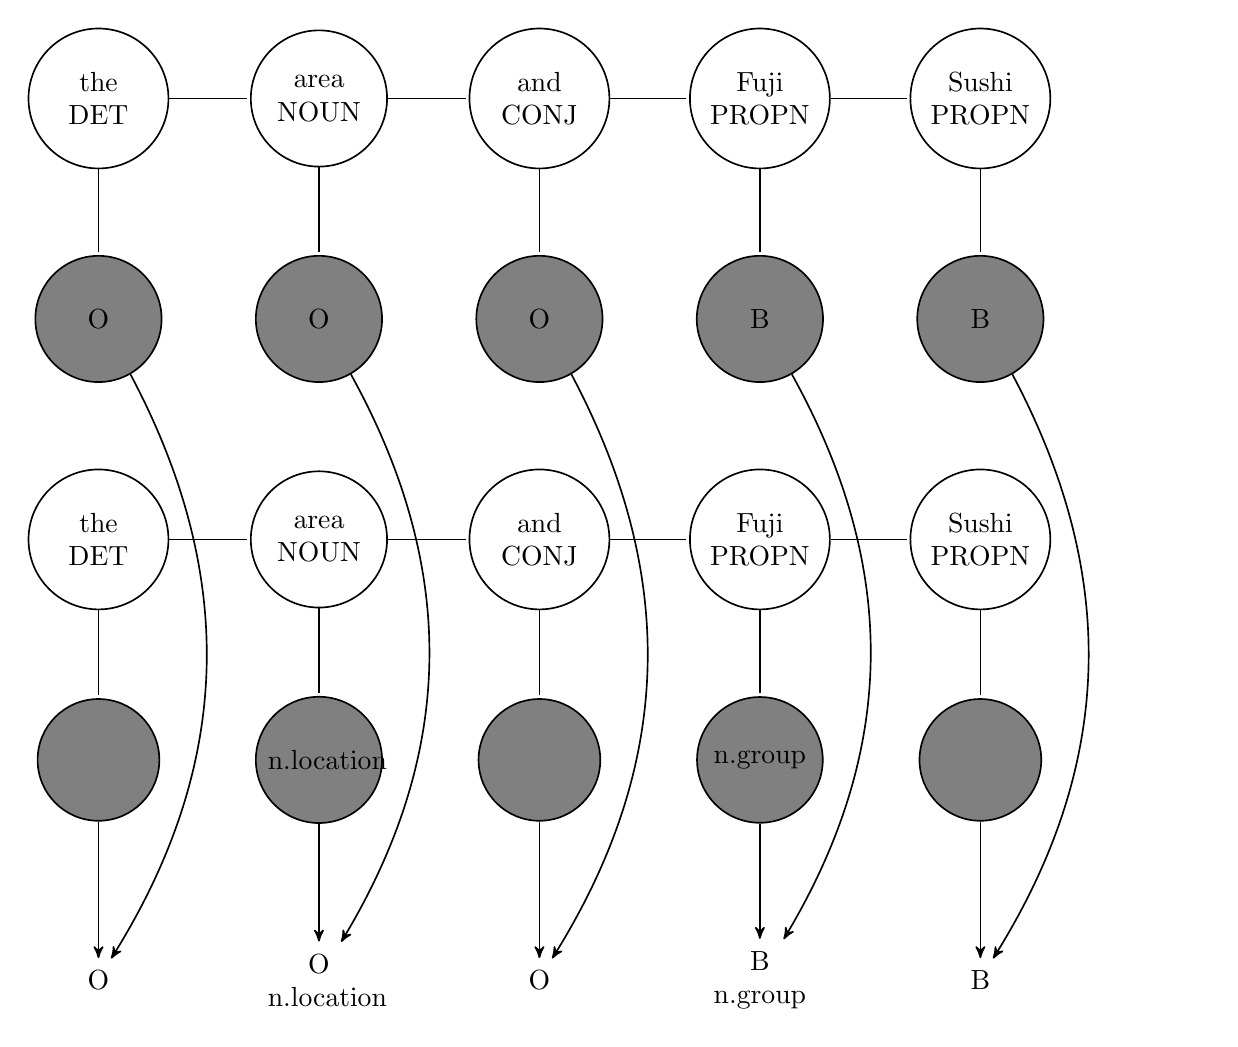
\begin{tikzpicture}[-,>=stealth',shorten >=1pt,auto,node distance=2.8cm,semithick,text width=1.3cm, align=center]
    \node[state] (A)              {the\\ DET};
    \node[state] (B) [right of=A] {area\\ NOUN };
    \node[state] (C) [right of=B] {and\\ CONJ };
    \node[state] (D) [right of=C] {Fuji\\ PROPN};
    \node[state] (E) [right of=D] {Sushi\\ PROPN};
    \node[state,fill=gray] (F) [below of=A] {O};
    \node[state,fill=gray] (G) [below of=B] {O};
    \node[state,fill=gray] (H) [below of=C] {O};
    \node[state,fill=gray] (I) [below of=D] {B};
    \node[state,fill=gray] (J) [below of=E] {B};

    \node[state] (K) [below of=F]  {the\\ DET};
    \node[state] (L) [below of=G] {area\\ NOUN};
    \node[state] (M) [below of=H] {and\\ CONJ};
    \node[state] (N) [below of=I] {Fuji\\ PROPN};
    \node[state] (O) [below of=J] {Sushi\\ PROPN};
    \node[state,fill=gray] (P) [below of=K] {};
    \node[state,fill=gray] (Q) [below of=L] {n.location};
    \node[state,fill=gray] (R) [below of=M] {};
    \node[state,fill=gray] (S) [below of=N] {n.group};
    \node[state,fill=gray] (T) [below of=O] {};

    \node (U) [below of=P] {O};
    \node (V) [below of=Q] {O\\ n.location};
    \node (W) [below of=R] {O};
    \node (X) [below of=S] {B\\ n.group};
    \node (Y) [below of=T] {B};

    % paths connecting inital CRF
    \path
    (A) edge              node {} (B)
    (A) edge              node {} (F)
    (B) edge              node {} (C)
    (B) edge              node {} (G)
    (C) edge              node {} (D)
    (C) edge              node {} (H)
    (D) edge              node {} (E)
    (D) edge              node {} (I)
    (E) edge              node {} (J);
    % path connecting both CRF layers
    \path[->]
    (F) edge [bend left]  node {} (U)
    (G) edge [bend left]  node {} (V)
    (H) edge [bend left]  node {} (W)
    (I) edge [bend left]  node {} (X)
    (J) edge [bend left]  node {} (Y)
    (P) edge              node {} (U)
    (Q) edge              node {} (V)
    (R) edge              node {} (W)
    (S) edge              node {} (X)
    (T) edge              node {} (Y);

    % paths for output CRF
    \path
    (K) edge              node {} (L)
    (K) edge              node {} (P)
    (L) edge              node {} (M)
    (L) edge              node {} (Q)
    (M) edge              node {} (N)
    (M) edge              node {} (R)
    (N) edge              node {} (O)
    (N) edge              node {} (S)
    (O) edge              node {} (T);

  \end{tikzpicture}
  \caption{CRF Baseline 2}
  \label{fig:crfbaseline2}
\end{figure}

\subsubsection{Baseline 3 Algorithm:}
The final baseline system uses a single CRF with joint MWE and Supersense labels. The predicted labels are then split after prediction. It provides a methodology for comparing ``jointness'' of tags and single CRF solutions. 

\begin{mdframed}[
    linewidth=0pt,
    roundcorner=4pt,
    backgroundcolor=gray!15,
    userdefinedwidth=\textwidth,
]
\begin{enumerate}
\tiny
  \setlength{\itemsep}{0pt}
  \setlength{\parskip}{0pt}
\item Extract features from training data with $\pm 2$ word context (Lemma+POS Tags)
\item Train CRF to predict concatenated MWE Tags and Supersense tags using features in (1)
\item Predict concatenated label sequences using (2)
\item Split MWE and Supersense sequences from (3)
\item Systematically create parent offset sequences for MWE sequences
\item Combine MWE and Supersense predictions in (4) with parent offset sequences in (5) for final predictions
\end{enumerate}
\end{mdframed}

The previous image defined in Figure \ref{fig:crfwindowgraydimsum} would be the corresponding diagram to baseline 3. A single CRF layer uses a windows of $\pm$2 and extracts the features of Lemma and POS tags to predict joint MWE and Supersense tags.

\subsection{Feature engineering}
For the baseline, three separate systems were created with different features for cross-comparison, allowing to correlate and contrast features against evaluation results. 

As spoken about in the previous chapter and shown in Figure \ref{fig:dimsumcolumns}, there are 9 columns of data in each sentence. Columns containing MWE, Parent offset indicies and Supersenses must be filled in by the prediction. Therefore columns 1,2,3 and 4 are available for feature engineering. They are the data corresponding to token offset, word, lowercase lemma and POS tag respectively. The obvious choices are word, lemma and POS tag since the token offset is an ambiguous per-line index. 

Using lemma and POS tags was the initial choice as they are less sparse then words. Conceptually, \texttt{Noun-Phrase} level MWEs are generally associated with Named Entities and have capitalised features. Using lemma and POS tags should generalise NER and other possible MWEs as well as capturing other Supersenses. 

Initial tests with Lemma and POS tags on varying window lengths show that F1-Score has a correlation to window size. Window boundaries were changed in equivalent lengths on each side of the input word. First the boundaries were set fixed to (-2,2) for Supersenses and MWE boundaries were increased, then evaluation of predicted results were captured. Similar tests were done by fixing the MWE boundaries (-2,2) and Supersense boundaries were increased followed by evaluation of the predicted results.

The length of the window is the absolute distance between the boundaries, or alternatively the quantity of tokens on either side of the input. Table \ref{tab:crfwinsizef1score} shows the F1-Score results for the window boundary changes. The values that are empty are due to failures in predictions for MWE sequences therefore evaluations were not available. 

The additional graph in Figure \ref{fig:crfwinsizef1score} is a visualisation of the data in Table \ref{tab:crfwinsizef1score}. The lower half shows the absolute distance, or windows length while the upper half shows the F1-Scores. As the MWE window size increases, there is little to no change in MWE F1-Scores, whereas when the Supersense window size increases, there is a decrease in F1-Scores. Setting the window size of $\pm$2 was chosen for both Supersense and MWE as it performed the best across all baseline systems. 

\newpage
\begin{table}[H]
\centering
\begin{tabular}{|cccc|ccc|}
\hline
\multicolumn{4}{|c|}{\bf Context Window} & \multicolumn{3}{c|}{\bf F1-Score Results}\\
\multicolumn{2}{|c}{MWE} & \multicolumn{2}{c|}{Supersense} &  &  &  \\
\hline
Boundaries & Length & Boundaries & Length & MWE & Supersense & Combined\\
\hline
-1,1 & 2 & -2,2 & 4 &  &  & \\
-2,2 & 4 & -2,2 & 4 & 37.37 & 45.83 & 44.68\\
-3,3 & 6 & -2,2 & 4 & 36.99 & 45.88 & 44.63\\
-4,4 & 8 & -2,2 & 4 &  &  & \\
-5,5 & 10 & -2,2 & 4 & 35.17 & 45.81 & 44.36\\
-6,6 & 12 & -2,2 & 4 & 34.46 & 45.68 & 44.15\\
-7,7 & 14 & -2,2 & 4 & 34.12 & 45.54 & 43.98\\
-8,8 & 16 & -2,2 & 4 & 34.33 & 45.66 & 44.1\\
-9,9 & 18 & -2,2 & 4 & 34.15 & 45.59 & 44.03\\
-2,2 & 4 & -1,1 & 2 & 37.37 & 47.09 & 45.76\\
-2,2 & 4 & -2,2 & 4 & 37.37 & 45.83 & 44.68\\
-2,2 & 4 & -3,3 & 6 & 37.37 & 44.83 & 43.81\\
-2,2 & 4 & -4,4 & 8 & 37.37 & 43.23 & 42.43\\
-2,2 & 4 & -5,5 & 10 & 37.37 & 43.15 & 42.36\\
-2,2 & 4 & -6,6 & 12 & 37.37 & 42.37 & 41.68\\
-2,2 & 4 & -7,7 & 14 & 37.37 & 41.79 & 41.18\\
-2,2 & 4 & -8,8 & 16 & 37.37 & 41.64 & 41.05\\
-2,2 & 4 & -9,9 & 18 & 37.37 & 41.10 & 40.59\\
\hline
\end{tabular}
\caption{CRF Window boundaries, Length and F1-Scores}
\label{tab:crfwinsizef1score}
\end{table}

\begin{figure}[H]
\centering
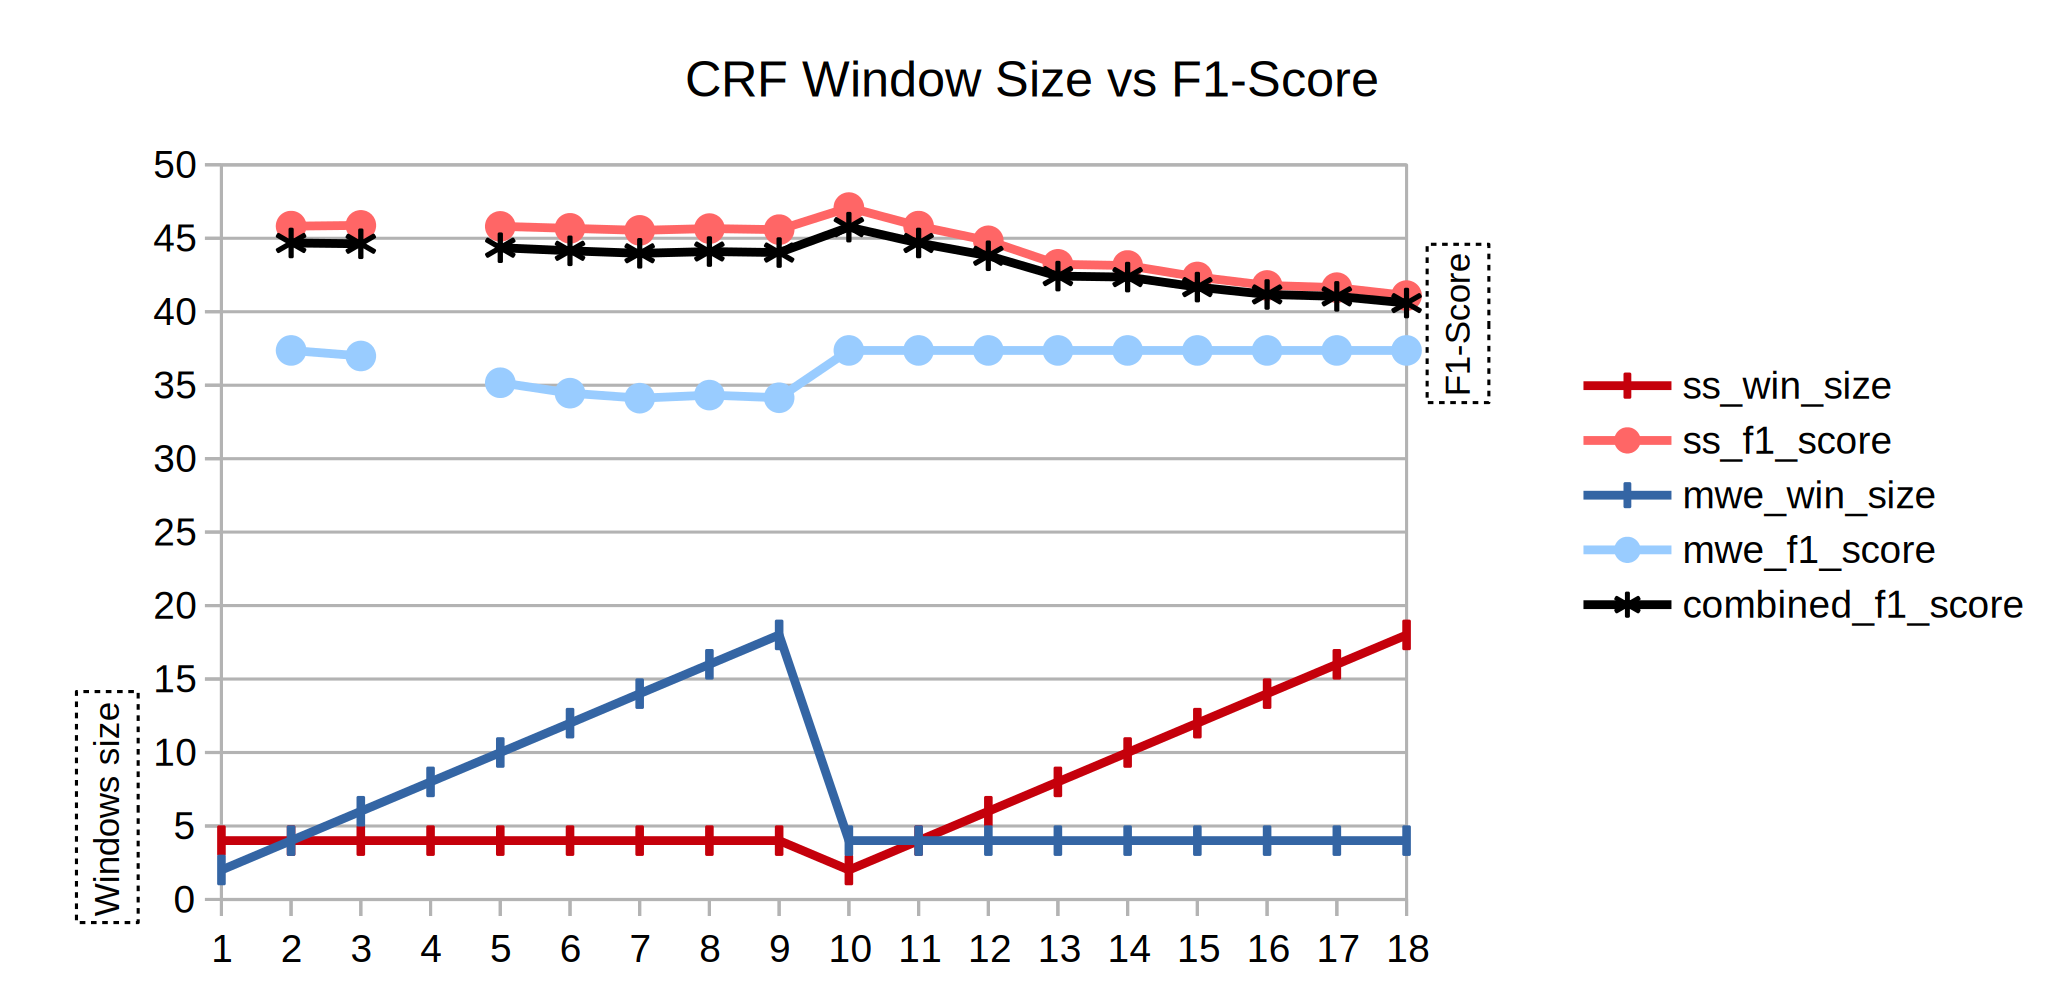
\includegraphics[width=\textwidth]{images/crf_win_size_f1_score.png}
\caption{CRF Windows size vs. F1-Score}
\label{fig:crfwinsizef1score}
\end{figure}

\subsection{Constraints and Evaluation}

To ensure valid constraints were upheld by baseline systems, MWE tag sequences were checked using a regular expression that was originally defined in the \texttt{dimsumeval.py} script. If an MWE sequence was found to be incorrect it would be modified by replacing the sequence with a valid sequence. Since a predictable substitution is not known, it is replaced with a sequence of \texttt{O} tags. Making this choice has a two-fold benefit, it creates a valid MWE sequence and it inherently fixes Supersense prediction locations when appearing on the incorrect corresponding MWE tags (such as \texttt{Ii}). Therefore the incorrectly assigned supersense as seen previously in Table~\ref{tab:supersensetagging} can never occur. 

The choice of this particular tag sequence is related to frequency of the presence of {\bf O}utside labels. The highest frequency label is the {\bf O}utside label and any sequence of continuous \texttt{O}s is considered valid. It also has the added benefit of not having supersense label restrictions as supersenses can only be associated with {\bf B}eginning labels. 

Quantifiable analysis on failures in MWE label prediction are covered in greater detail in Section \ref{chapter5discussionpitfalls}. 

\section{Bi-LSTM-CRF Solution}

Using an Recurrent Neural Network system over a pure Conditional Random Field solution has the benefit of substituting feature engineering for network architecture. It potentially introduces a more generalisable data-driven approach over a hand-crafted one. Albeit preferable to have a simple solution, exploiting the data for the task will produce more coherent results.

Basic RNNs have been used in almost any NLP related task with varying success. In this task we try to use the sequential nature of a bidirectional LSTM which will give us the flexibility of our original CRF on any given input. A final CRF output layer is used for predicting labels using Bi-LSTM outputs as features. Word embeddings are used as input features to the Bi-LSTM to broaden scope to the ``open'' data condition and improve results.

\begin{figure}[H]
\centering
\includegraphics[width=0.8\textwidth]{images/LSTM_CRF_inkscape.png}
\caption{LSTM-CRF Example with \dimsum data inputs}
\label{fig:lstmcrfexampledimsumdata}
\end{figure}

\subsection{Code Adaption}

A NER tagging solution was created in the publication \cite{Lample2016} using a Bi-LSTM-CRF for CoNLL sentence data. A code adaption for the \dimsum task was done by modifying their \texttt{tagger} solution which can be found at {\url{https://github.com/glample/tagger}} \cite{githubglampletagger}. The updated fork modified for the \dimsum task can be found at {\url{https://github.com/natemccoy/tagger}} \cite{githubnatemccoytagger}.

The original task predicted only \texttt{BIO} tags and was trained on Reuters RCV1 data set which requires a license to use. The adaption uses only publically available data. It uses pre-processed \dimsum data \cite{dimsum16webdata} and Google News's pre-trained word vectors available on the \texttt{word2vec} website \cite{word2vecgooglecodeweb}.

\subsection{Joint Labels}

Baseline results as seen in Chapter \ref{chapter5} prove that Joint labels produced the highest combined F1-Score. The ``jointness'' of tags captures relationships that are otherwise misclassified during prediction time. Therefore a joint tag solution is created using the adapted code. 

Post-processing of joint tags is done after prediction to split predicted labels and evaluate results. The adaption therefore predicts single joint labels for a given input sentence.

The positive aspect of joint tag prediction is the elimination of supersense constraint violations. No supersense is predicted on a MWE tag that is not \texttt{[B|b]}. Alternatively, the cons are that it still may produce incorrect MWE sequences. 

\subsection{Features}
When speaking about features, we do not intend to speak about feature engineering as it is absent from the adapted model. Rather, the design of the adapted code has specific hyperparameters and a construction which allows for additional flexibility such as pre-embeddings.

\subsubsection{Bidirectionality}\label{featurebidirectionality}

As proposed by \cite{schuster1997bidirectional} and demonstrated by \cite{Sutskever2014} and \cite{Graves2005}, bidirectional LSTMs increase performance over traditional LSTMs. Single directional LSTMs capture shorter-range dependencies as they ``forget'' long-range dependencies over time. Bidirectional LSTMs account for long-range dependencies in past and future ``memory'' inputs. This is achieved by using forward and reverse direction LSTMs to capture past and future dependencies for a given input. 
The Bi-LSTM-CRF uses bidirectional features for word and character. This means that weights are initialised to the dimension defined during training then \texttt{\underline{L}}eft and \texttt{\underline{R}}ight LSTMs are concatenated to create a more temporally robust input vector for the CRF layer as seen in Figure \ref{fig:lstmcrfexampledimsumdata}.

\subsubsection{Pre-embeddings}

Pre-computed embedding vectors can be used during training. If no pre-embedded vectors are supplied they are initialised at random and trained. Significant increases in performance are gained by using pre-embeddings as shown in the original NER tagger that was adapted for this task \cite{Lample2016} and which will be demonstrated in the following chapters. The pre-embedded vectors used were taken from the \texttt{GoogleNews-negative300.bin} which are available at \cite{word2vecgooglecodeweb}.

\subsubsection{Character embeddings}
Character level embeddings are somewhat new when it comes to MWE related tasks. As shown by the original Bi-LSTM-CRF \texttt{tagger} implementation in \cite{Lample2016} and similar research by \cite{Chiu2015}, character level embeddings capture details important to MWE and NER tasks. Many MWEs are Named entities and can exploit the use of character level information in disambiguating labels. Upper and Lower case features as well as punctuation marks in specific sequences can help determine a label for a given input. 
A character level LSTM is used in the Bi-LSTM-CRF so exploit these details. As spoken about in the Analysis section in Chapter \ref{chapter3}, a sizeable amount of MWE tagged heads have the POS tag NOUN or PROPN. Therefore capturing features on a character level can help determine correct labels in the \dimsum data. 

\subsubsection{Hyperparameters}

As briefly mentioned in the section \ref{featurebidirectionality}, word and character bidirectionality dimensions can be chosen at training time as well as, dropout rate, optimisation method and learning rate. Smaller character dimensions gave better results. Stochastic gradient descent with a learning rate of 0.005 gave the best results which were also the original default settings.

\subsection{Constraints and Evaluation}

In few occasions, MWE tags were predicted incorrectly but were fixed in the same methodology used for the CRF baselines by substituting the MWE tag sequence with {\bf O}utside tags equivalent to the sequence length. This issue is independent of supersenses being predicted on non-\texttt{B} labels as the system uses joint labels therefore enforcing the {\bf B}eginning+Supersense constraint when applicable. The evaluation results of the modified sequences will be spoken of in greater detail in Chapter \ref{chapter5} in the pitfalls section \ref{chapter5discussionpitfalls}.

\chapter{Results and Discussion}\label{chapter5}

In this chapter we will demonstrate the results succeeded in proving the experiments were a success on the \dimsum task. Both the baseline and final systems provided solutions to the task while the Bi-LSTM-CRF outperformed the baseline.

The results section \ref{chapter5results} will mention the CRF baseline results and Bi-LSTM-CRF final results. Data splits will be briefly mentioned and can be read about in more details in the data section of the appendix \ref{appendixdata}. Epoch cutoffs are established and used for the final Bi-LSTM-CRF results and will be demonstrated. Final results for both systems will be compared.

The Discussion section will speak about comparisons of results with the original task publication, move on to the pitfalls of the design and finally discuss possible improvements for future work.

\section{Results}\label{chapter5results}
To ensure high quality results and remove ``contamination'' of testing data while training solutions, additional data splits were created from \dimsum task corpus. The data splits were used mainly for the Bi-LSTM-CRF but were nonetheless important in establishing a rigorous methodology for model training and comparisons. The \texttt{dimsum16.train} file was split into separate \texttt{train/dev/test} sets by percentages of \texttt{60/20/20} and \texttt{80/20/-} respectively. For more details on the data please refer to the appendix \ref{appendixdata}.

An example how evaluation is performed with additional images showing a misaligned prediction with supersense errors can be seen in Figure \ref{fig:linkmeasure} which was taken directly from the original \dimsum publication \cite{Schneider2016}.

\newcommand{\tagtss}[5]{\begin{tabular}{@{\hspace{2pt}}c@{\hspace{2pt}}} \texttt{#2\vphantom{\textlarger{Ĩ}}}\\ \sst{#3}\vphantom{X} \\ \textbf{#1}\vphantom{lp} \\ \sst{#5}\vphantom{X} \\ \texttt{#4\vphantom{\textlarger{Ĩ}}}\end{tabular}}
\newcommand{\sst}[1]{\textsc{#1}} % supersense category
\begin{figure}[H] %\small
% {``34'': [``price'', ``POSSESSION''], ``36'': [``means'', ``cognition''], ``26'': [``was'', ``stative''], ``29'': [``budge'', ``change'']}
\begin{framed}\small
\emph{MWE Precision:} The proportion of predicted links whose words 
both belong to the same expression in the gold standard. \\
\emph{MWE Recall:} Same as precision, but swapping the predicted and gold annotations. %\\
%\emph{Strength Averaging:} A weak link is treated as intermediate between a strong link and no link at all: 
%precision, recall, and $F_1$ computed on strong links only are averaged 
%with the respective calculations computed on all links without regard to strength.
\end{framed}\centering
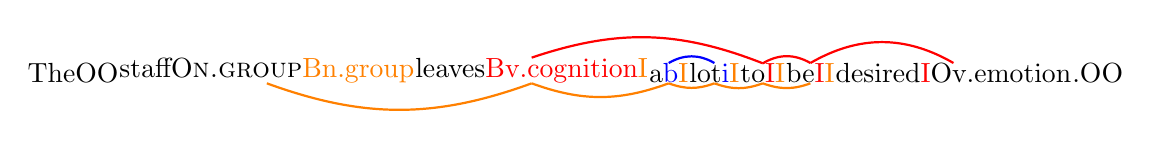
\begin{tikzpicture}[baseline={($(current bounding box.center)+(0,-0.5ex)$)}, node distance=0cm, auto,]
 \node[inner sep=0cm]                                  (n1) {\tagtss{The}{O}{}{O}{}};
 \node[inner sep=0cm,above right=0pt of n1.south east] (n2) {\tagtss{staff}{O}{\textsc{n.group}}{\color{orange}B}{\color{orange}n.group}};
 \node[inner sep=0cm,above right=0pt of n2.south east] (n3) {\tagtss{leaves}{\color{red}B}{\color{red}v.cognition}{\color{orange}I}{}};
 \node[inner sep=0cm,above right=0pt of n3.south east] (n4) {\tagtss{a}{\color{blue}b}{}{\color{orange}I}{}};
 \node[inner sep=0cm,above right=0pt of n4.south east] (n5) {\tagtss{lot}{\color{blue}i}{}{\color{orange}I}{}};
 \node[inner sep=0cm,above right=0pt of n5.south east] (n6) {\tagtss{to}{\color{red}I}{}{\color{orange}I}{}};
%\path[-,thick,dotted, bend left=30] (n2.north) edge (n3.north); 
\path[-,thick,red, bend left=20] (n3.north) edge (n6.north);
 \path[-,thick,blue, bend left=30] (n4.north) edge (n5.north);
\path[-,thick,orange, bend right=20] (n2.south) edge (n3.south);
\path[-,thick,orange, bend right=20] (n3.south) edge (n4.south);
\path[-,thick,orange, bend right=20] (n4.south) edge (n5.south);
\path[-,thick,orange, bend right=20] (n5.south) edge (n6.south);
 \node[inner sep=0cm,above right=0pt of n6.south east] (n7) {\tagtss{be}{\color{red}I}{}{\color{orange}I}{}};
\path[-,thick,orange, bend right=20] (n6.south) edge (n7.south); 
 \node[inner sep=0cm,above right=0pt of n7.south east] (n8) {\tagtss{desired}{\color{red}I}{}{O}{v.emotion}};
\path[-,thick,red, bend left=30] (n6.north) edge (n7.north);
\path[-,thick,red, bend left=30] (n7.north) edge (n8.north);
 \node[inner sep=0cm,above right=0pt of n8.south east] (n9) {\tagtss{.}{O}{}{O}{}};
\end{tikzpicture}
\caption{A \textsc{Reviews} sentence with MWE and supersense analyses: gold above and hypothetical prediction below. 
MWE precision of the bottom annotation relative to the top one is $2/5$. %with weak links removed 
%and $2/6$ with weak links strengthened to strong links
(Note that a link between words $w_1$ and $w_2$ is ``matched'' 
if, in the other annotation, there is a path between $w_1$ and $w_2$.) 
The MWE recall value is $3/4$. 
Supersense precision and recall are both $1/2$.
Combined precision/recall scores add the respective subscores' numerators and denominators:
thus, combined precision is $\tfrac{2+1}{5+2} = 3/7$, 
and combined recall is $\tfrac{3+1}{4+2} = 2/3$.
Combined $F_1$ is their harmonic mean, i.e.~$12/23$.
%Overall $F_1$ is computed as the average of two $F_1$-scores, i.e.~$\tfrac{1}{3} \cdot \tfrac{1}{1}/(\tfrac{1}{3} + \tfrac{1}{1}) + \tfrac{2}{6}\cdot \tfrac{3}{3}/(\tfrac{2}{6}+\tfrac{3}{3}) = 0.50$.
}
\label{fig:linkmeasure}
\end{figure}

All final results are compared using F1-Scores from the \dimsum task's provided evaluation script \texttt{dimsumeval.py} to establish a framework for relational comparability. Additional results for precision, recall and accuracy will be presented for completeness.

\subsection{CRF Baselines}

Evaluation results are computed by using a combined mean of Recall, Precision, F1-Score and Accuracy for MWE and Supersense predictions. 

The combined score represents the averaged predictive results as seen in Figure \ref{fig:baselinescombinedresults}. For more verbose details on individual results please refer to the appendix \ref{appendixresults}.

\begin{figure}[H]
  \begin{minipage}{.5\textwidth}
    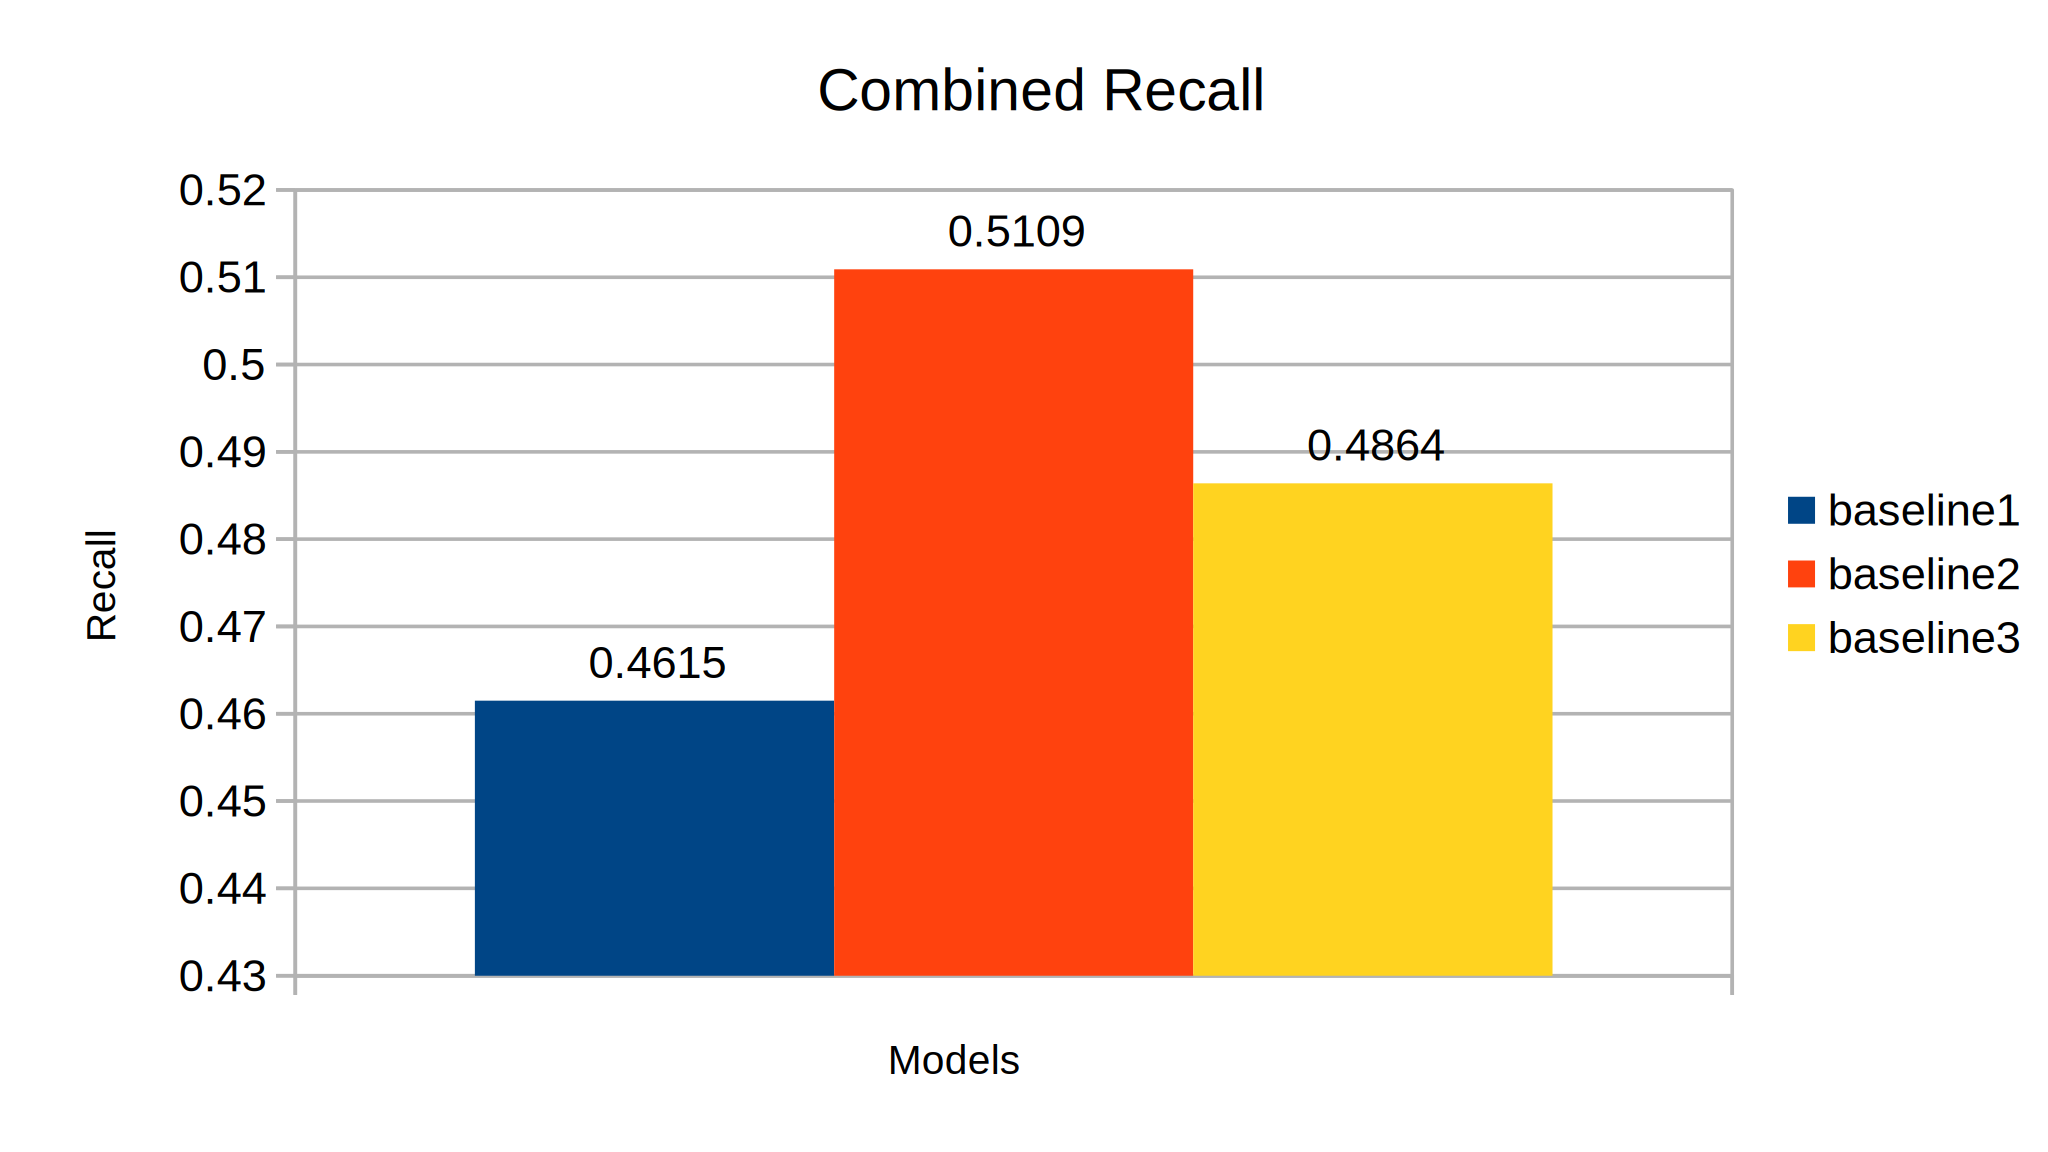
\includegraphics[width=\textwidth]{images/baselines_combined_recall.png}
    \centerline{Recall}\medskip
  \end{minipage}\hfill
  \begin{minipage}{.5\textwidth}
    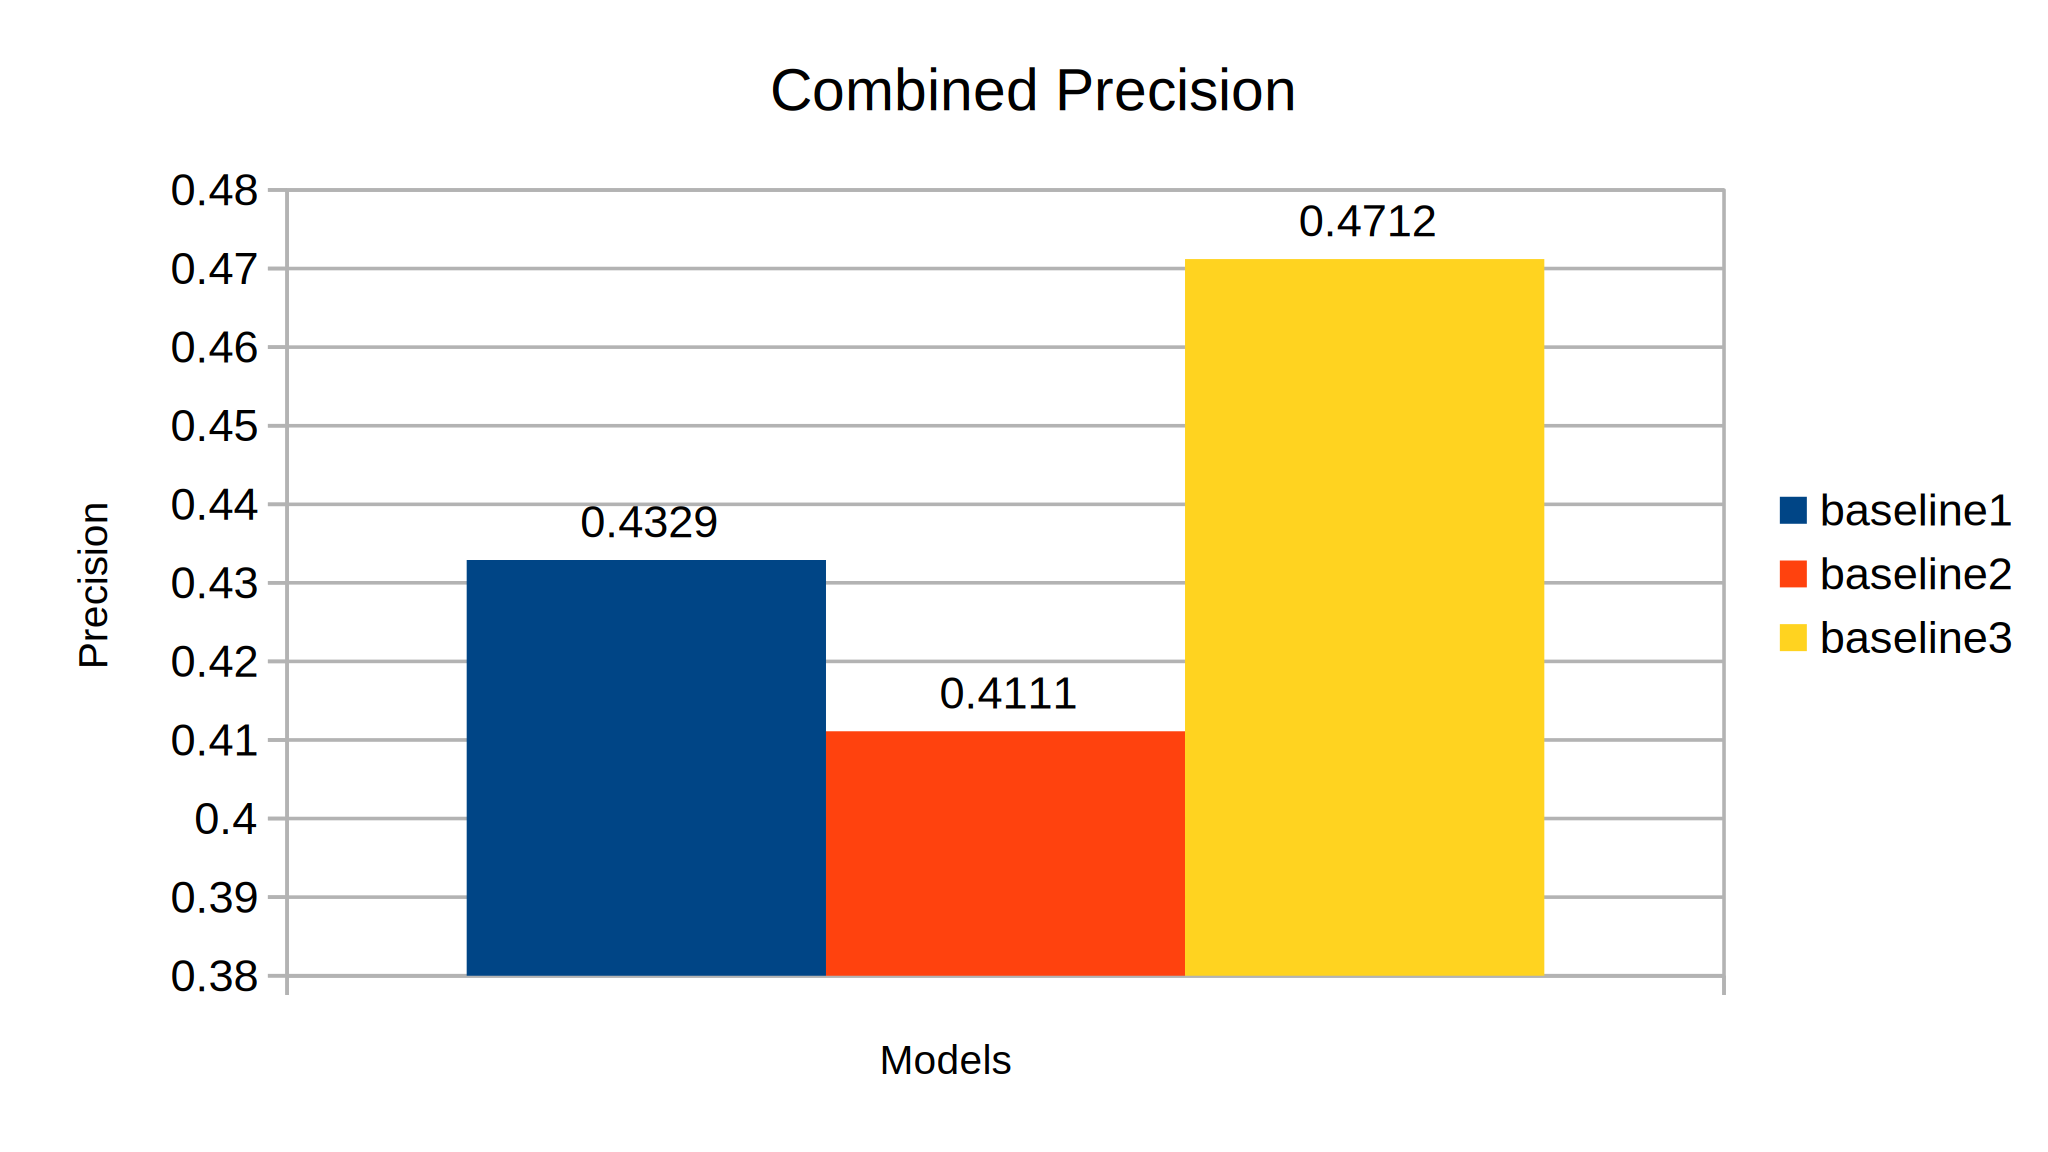
\includegraphics[width=\textwidth]{images/baselines_combined_precision.png}
    \centerline{Precision}\medskip
  \end{minipage}\\
  \begin{minipage}{.5\textwidth}
    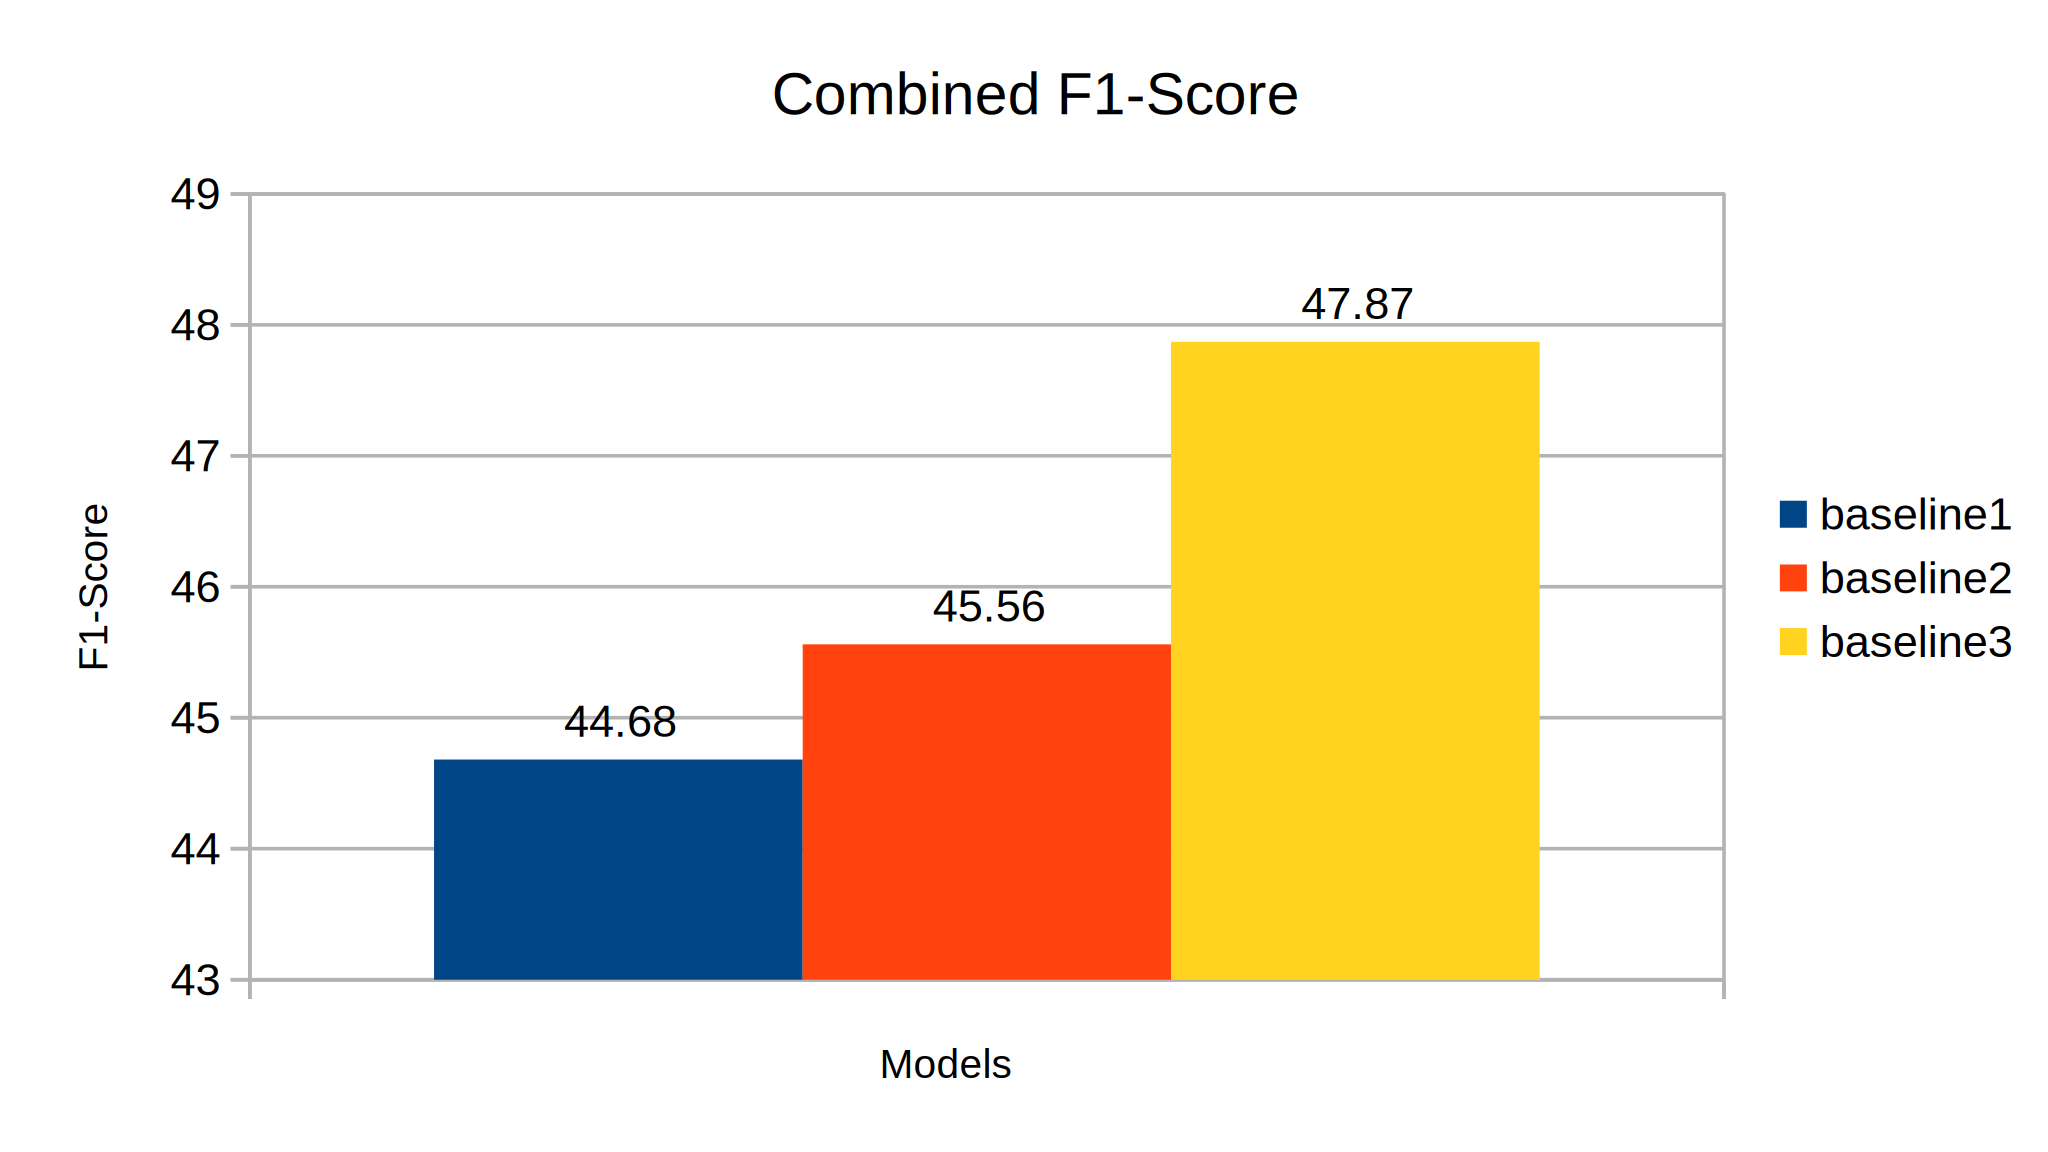
\includegraphics[width=\textwidth]{images/baselines_combined_f1score.png}
    \centerline{F1-Score}\medskip
  \end{minipage}\hfill
  \begin{minipage}{.5\textwidth}
    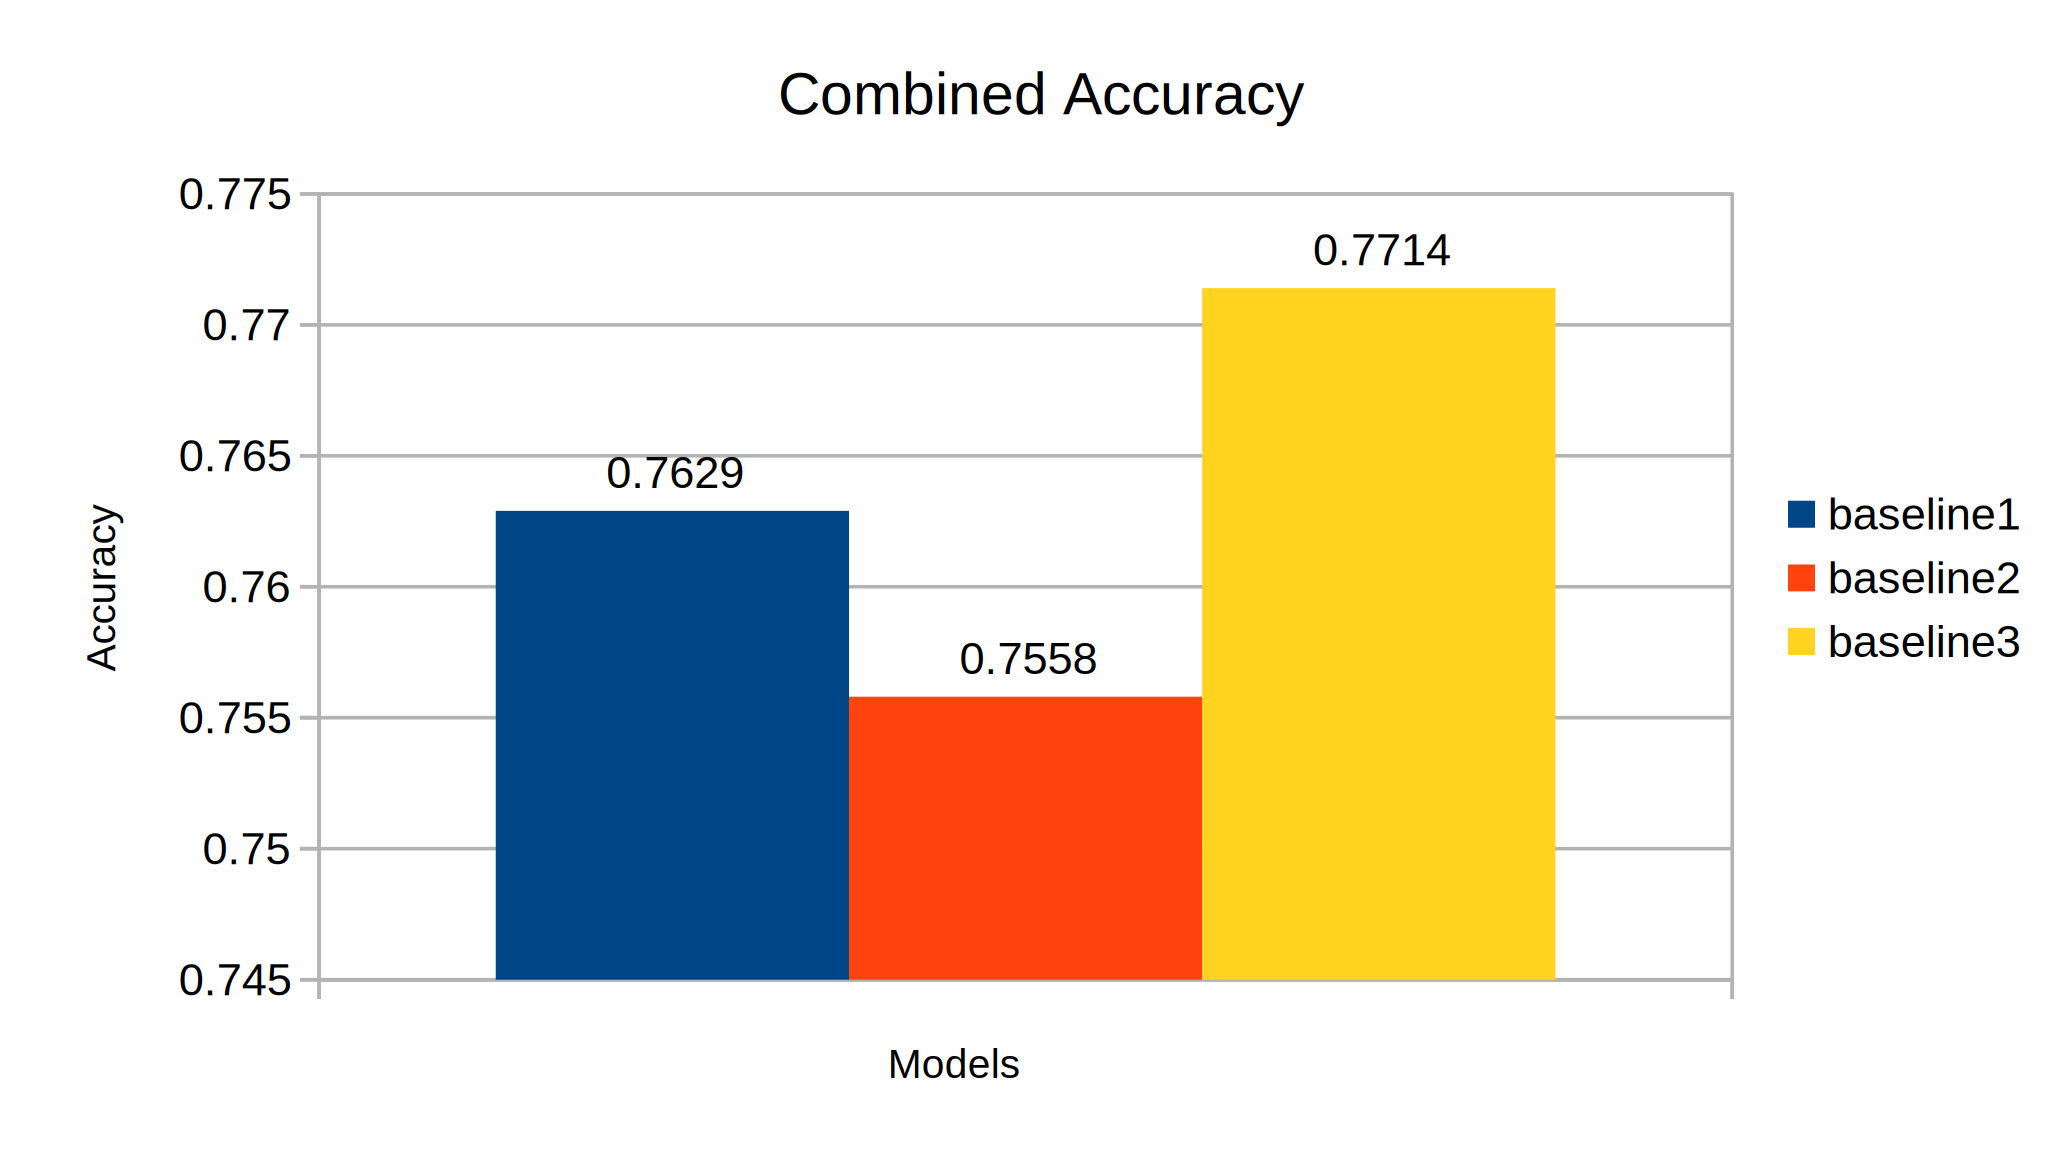
\includegraphics[width=\textwidth]{images/baselines_combined_accuracy.png}
    \centerline{Accuracy}\medskip
  \end{minipage}\\
  \begin{minipage}{\textwidth}
    \centerline{\includegraphics[width=0.7\textwidth]{images/baselines_combined_legend.png}}
  \end{minipage}
  \caption{Baselines Combined Results}
  \label{fig:baselinescombinedresults}
\end{figure}

The results for the baseline systems show that baseline number 3 produced a quantifiably higher result in all areas except Recall. The combined average F1-Score for baseline number 3 produced a 2.3\% increase over baseline 2 and 3.1\% increase over baseline 1. For this reason baseline number 3 was considered to be the best baseline for the \dimsum task. The characteristic difference was joint tags which directly lead to the correlation of ``jointness'' as the most influential aspect in performance.

\subsection{Bi-LSTM-CRF}
The use of the \texttt{60/20/20} data split from \texttt{dimsum16.train} was used for parameter optimisations to ensure complete separation from the \texttt{dimsum16.test} data, which was only used for the final results. 

During these initial tests, default parameters were used to determine epoch limitations. The default epoch limit was set to 100 but upon review of \texttt{dev} and \texttt{test} evaluations, over-fitting can be observed by around the 25th epoch as seen in Figure \ref{fig:bilstmcrfepochcutoff}. To save time for subsequent optimisation tests, a limit of 25 epochs was chosen for training. 

\begin{figure}[H]
\centering
\includegraphics[width=0.8\textwidth]{images/bi_lstm_crf_60_20_20_defaults_epoch_cutoff.png}
\caption{Bi-LSTM-CRF Epoch Cutoff}
\label{fig:bilstmcrfepochcutoff}
\end{figure}

Over 100 separate tests were done in order to optimise parameters for training on the \dimsum data \footnote{Appendix \ref{appendixresults} contains full table of training model results}. Training the optimised models took around 2 to 4 hours to complete on the university's computing cluster \texttt{iceberg}.

The final results using the \texttt{80/20/-} split with \texttt{dimsum16.test.blind} can be seen in Figure \ref{fig:bilstmcrfresults} where the leftmost line graph displays an average of F1-Score's over epochs and the rightmost bar graph shows the MWE, Supersense and Combined F1-Scores for the final trained model. 
\begin{figure}[H]
  \begin{minipage}{.5\textwidth}
    \includegraphics[width=\textwidth]{images/bi_lstm_crf_80_20_final_epochs_line_graph.png}
    \centerline{\footnotesize Training epochs F1-Scores}\medskip
  \end{minipage}\hfill
  \begin{minipage}{.5\textwidth}
    \includegraphics[width=\textwidth]{images/bi_lstm_crf_80_20_final_f1scores_bar_graph.png}
    \centerline{\footnotesize Testing MWE, Supersense and Combined F1-Scores}\medskip
  \end{minipage}\\
  \caption{Bi-LSTM-CRF Results}
  \label{fig:bilstmcrfresults}
\end{figure}

As demonstrated graphically, the final results are a combined F1-Score of 53.27\% which is a 5.4\% increase over the highest scoring baseline. Additional details about contributing factors to results will be mentioned in the discussion section \ref{chapter5discussion}.

\subsection{Comparisons}\label{chapter5resultscomparisons}
A comparison of results obtained from evaluations of CRF baselines, Bi-LSTM-CRF and published results from \cite{Schneider2016} will be presented in this section.

The original publication used team names and system numbers prefixed with ``\texttt{S}'' to distinguish solution submissions for the \dimsum task. In the table below, all results are shown from the original publication compared to the CRF Baseline systems and the final Bi-LSTM-CRF evaluation results. 
\begin{figure}[H]
  \begin{minipage}{\textwidth}
    \centering
    \begin{tabular}{|l|l|l|l|}
      \hline
      \textbf{System} & \textbf{Team}  & \textbf{Score} & \textbf{Resources}\\
      \hline
      \hline
      \texttt{S214} & ICL-HD & 57.77 & ++ \\
      \hline
      \texttt{S249} & UW-CSE & 57.71 & ++ \\
      \hline
      \texttt{S248} & UW-CSE & 57.10 &    \\
      \hline
      \texttt{\it Bi-LSTM-CRF} & & \hl{\bf 53.27} & ++ \\
      \hline
      \texttt{S106} & UFRGS\&LIF & 50.27 &   \\
      \hline
      \texttt{S227} & VectorWeavers & 49.94 & ++ \\
      \hline
      \texttt{\it CRF Baseline 3} & &  47.87 &   \\
      \hline
      \texttt{S255} & UTU & 47.13 & ++ \\
      \hline
      \texttt{S211} & UTU & 46.17 & + \\
      \hline
      \texttt{S254} & UTU & 45.79 &   \\
      \hline
      \texttt{\it CRF Baseline 2} & & 45.56 &   \\
      \hline
      \texttt{\it CRF Baseline 1} & & 44.68 &   \\
      \hline
      \texttt{S108} & WHUNlp & 25.71 &   \\
      \hline
    \end{tabular}
  \end{minipage}\\
  \begin{minipage}{\textwidth}
    \includegraphics[width=\textwidth]{images/systems_comparison_bar_graph.png}
  \end{minipage}
  \caption{System F1-Scores Comparison}
  \label{fig:systemsf1scorescomparison}
\end{figure}

The team name for the results is the author's name shown in italics while the highest scoring solution created for this dissertation is highlighted and printed in bold. All data is provided from highest scoring systems to lowest. 

In addition, Figure \ref{fig:systemsf1scorescomparison} shows a bar graph to demonstrate the data in an alternative manner with the four systems created for this dissertation coloured in while the original publication's results are shown in black and white with varying hatch marks only. 

The plus symbols are used to describe the data condition types (as mentioned in Chapter \ref{chapter3}) which are ``supervised closed'', ``semi-supervised closed'' and ``open''\footnote{As stated in \cite{Schneider2016}, ``The final column indicates the resource condition: systems entered in the open condition (all resources allowed) are designated “++”; “+” indicates the more restricted semi-supervised closed condition, while the remaining systems are in the closed condition (most restrictive).''}. The baseline systems used the most restrictive condition of supervised closed, using only the data provided for the original \dimsum task. Due to the usage of the pre-computed word embeddings, the final Bi-LSTM-CRF is considered to be in the least restrictive data condition category of ``open''.

\section{Discussion}\label{chapter5discussion}
A reflection of system capabilities is paramount to understanding quantifiable scientific findings after an evaluation has been performed. Self-examination and critique allows for further work to be developed and possible additions to be made to increase performance. This section intends to speak about intrinsic evaluation findings and potential pitfalls of the systems developed. By making such a critique, improvements will be considered for future enhancements and adaptions.  

For the most part, the discussion will be focused on the final result using the Bi-LSTM-CRF. The observations, pitfalls and improvements will cover the final model's approach to the \dimsum task.

\subsection{Intrinsic observations}
Some observations during the Bi-LSTM-CRF optimisation are notable for different reasons, but are mainly considered important for future developments using a similar model. A couple interesting points will be presented here. 

\subsubsection{CRF Layer}

The final layer of the Bi-LSTM-CRF as seen in Figure \ref{fig:lstmcrfexampledimsumdata} shows a final output CRF layer. This layer can be disabled in the adapted code, and during the optimisation process it was one of the tests that was performed. The joint tag predictions were based only on the combined Bi-LSTM output. As seen in Figure \ref{fig:602020crflayerenabledisablelinegraph}, a clear difference between the usage of the CRF layer to encode contextual information can be seen to be beneficial. The upper most lines show the CRF layer enabled and the bottom most lines show the CRF layer disabled demonstrated by using the plus and minus symbols for enabled and disabled respectively. The tests were done using the \texttt{60/20/20} data split from \texttt{dimsum16.train}. The first few epochs when disabling the CRF layer has some missing data points due to precision or recall being zero which lead to 'nan' values for F1-Scores.

\begin{figure}[H]
  \includegraphics[width=\textwidth]{images/bi_lstm_crf_60_20_20_crf_comparison_training_line_graph.png}
  \caption{60/20/20 Training epochs for CRF Layer Enabled/Disabled}
  \label{fig:602020crflayerenabledisablelinegraph}
\end{figure}

The difference between disabling and enabling the CRF layer is about 24 to 28 percent for test and dev respectively using the \texttt{60/20/20} split during training. By disabling the CRF layer in the code, you remove the additional power of the CRF which uses transitions and observation compiled by the training data to determine the most likely joint tag candidate. 

Training and testing with the \texttt{80/20/-} split and testing with the \texttt{dimsum16.test.blind} shows similar results as seen in Figure \ref{fig:8020crflayerenabledisablebargraph} with a difference of 21\% between disabling and enabling the CRF Layer.

\begin{figure}[H]
  \includegraphics[width=\textwidth]{images/bi_lstm_crf_80_20_crf_comparison_test_bar_graph.png}
  \caption{80/20 Test results for CRF Layer Enabled/Disabled}
  \label{fig:8020crflayerenabledisablebargraph}
\end{figure}

The use of the CRF in both models cannot be directly correlated as the features are not comparable. That being said, it can be argued that using the Bi-LSTM without the CRF layer for the \dimsum task cannot outperform a simple single CRF solution for joint tag prediction as seen in CRF baseline 3. An alternative configuration with different Bidirectional features may prove otherwise, but in it's current configuration the CRF layer is a valuable addition to the model even though it's true importance, either temporal or other, is not known. 

\subsubsection{Pre-embeddings}

The single most important optimisation to the model was using pre-embeddings. As seen in Figure \ref{fig:preembcomparison}, the performance gain jumped from 44.31\% to 53.27\% providing a 8.96\% increase over the same optimised model without pre-embeddings\footnote{Initial few epochs without pre-embeddings provided \texttt{nan} F1-Scores}.

\begin{figure}[H]
  \begin{minipage}{.5\textwidth}
    \includegraphics[width=\textwidth]{images/bi_lstm_crf_80_20_preembeddings_comparison_line_graph.png}
    \centerline{\footnotesize Training epochs F1-Scores}\medskip
  \end{minipage}\hfill
  \begin{minipage}{.5\textwidth}
    \includegraphics[width=\textwidth]{images/bi_lstm_crf_80_20_preembeddings_comparison_bar_graph.png}
    \centerline{\footnotesize Testing Combined F1-Scores}\medskip
  \end{minipage}\\
  \caption{Pre-embeddings comparison}
  \label{fig:preembcomparison}
\end{figure}

Most likely the pre-computed word embeddings provided much richer contextual detail to the input word vectors which was the key factor in boosting performance. These findings seem to be in line with other observations as seen in \cite{Schneider2016}.

\subsection{Pitfalls}\label{chapter5discussionpitfalls}

Critiquing the systems and data design can help determine failures in models and assumptions about data. This section intends to speak about both with specific attention to data usage.

\subsubsection{Joint tags as Predictive labels}
The final Bi-LSTM-CRF system uses labels read from training data. There are benefits and issues for this model. 

Using joint tags eliminated issues in prediction where {\bf B}eginning MWE tags were not coupled with supersenses, as all potential combinations in the training data inherently followed the structural limitation of MWE \texttt{[B|b]} and supersense tag coupling.

Every system designed has instances in which the MWE tags \texttt{{BbIiOo}}, were predicted in an invalid way, e.g. a sequence of only \texttt{I} labels without a \texttt{B}. In the majority of cases the {\bf B}eginning tags \texttt{[B|b]} were predicted in a wrong location or not predicted at all. This would mean that in a joint tag system, the only potential limitation would be failures in MWE tag prediction. Issues in regards to MWE tag prediction are spoken of more in the following section \ref{pitfallsmwes}.

The final Bi-LSTM-CRF model used, determines possible labels during training by reading data only, and not using a predefined set. One issue involved in using joint tags as predictive labels in the current configuration is that not all joint tags can be known from the training data. 

There are 6 possible tags for MWE tag sequences and 41 possible tags for Supersenses\footnote{the WordNet Supersense \texttt{n.Tops} is not used, otherwise there would be 42 possible Supersenses.} as seen in Section \ref{tab:wordnetsupersenses}. The cross product would give us a quantity of 246 possible tags. 

\begin{align*}
   |\{BbIiOo\}| \times |\{Supersenses\}| = 246
\end{align*}

In the \texttt{dimsum16.train} file only 118 joint tags can be constructed from reading the data alone. This means only 47\% of the possible joint tag labels are represented as seen in Table \ref{tab:jointtagcountsrepresented}.

\begin{table}[H]
    \centering
    \begin{tabular}{l|l|l}
      Cross-product Maximum & 246 & {\bf Total represented}\\
      \hline
      dimsum16.train & 118 & 47.07\%\\ 
      dimsum16.test & 90 & 36.59\%\\ 
    \end{tabular}
  \caption{Joint tag label counts with percent represented in data}
  \label{tab:jointtagcountsrepresented}
\end{table}

The benefit of creating a predictive label set from training data is flexibility, and that the system can work with minimal alterations for new labels. The downside is all of the unseen labels are mapped to the most frequent label, in our case the {\bf O}utside tag with no supersense.  

In our test data there are 90 joint tags and only 3 are not seen in the training data. Each of the 3 joint tag labels is seen only once. Therefore by predicting the highest probable joint tag label of ``\texttt{O\_\_}'' we introduce a negligible error. It these default labels introduced a complete MWE tag sequence error, it could only possibly decrease accuracy for MWE tag sequences by a maximum of 0.3\%.

All this being said, to make a more robust system, there should be a better way for handling unknown labels, such as giving the system the full set of possible labels beforehand. 

\subsubsection{MWEs}\label{pitfallsmwes}

The quantity of MWE tag sequences found to be invalid were only 16 in CRF Baseline 3 and 21 in the optimised Bi-LSTM-CRF. There were only 1000 test sentences so there was a total of 1.6\% to 2.10\% invalid MWE sequence predictions for CRF Baseline 3 and the optimised Bi-LSTM-CRF respectively. This can obviously be improved but shows that ``patching'' invalid sequences with \texttt{O} tag sequences can only introduce a 1.6-2.1\% error.

Interestingly enough, the valid sequences of sequential {\bf O}utside tags were about 14\% to 18\% of the MWE tag sequences that were predicted incorrectly as seen in Table \ref{tab:inseqoutmwetagseq}. 

\begin{table}[H]
    \centering
    \begin{tabular}{ll}
      Baseline 3 & Bi-LSTM-CRF\\
      \hline
      146 / 1000 & 186 / 1000\\
      14.6\% & 18.6\%
    \end{tabular}
  \caption{Incorrect Sequential {\bf O}utside MWE tag sequence}
  \label{tab:inseqoutmwetagseq}
\end{table}

This means that up to 18\% of incorrect MWE tag sequences had no MWEs predicted when they should have been. 

In a strictly accuracy based sense for entire MWE tag sequences, without regard to alignment or quantity of MWEs, there are a total of 480 and 492 invalid MWE tag sequences as seen in Table \ref{tab:accuracyinvalidtagseq}. 

\begin{table}[H]
    \centering
    \begin{tabular}{ll}
      Baseline 3 & Bi-LSTM-CRF\\
      \hline
      480 / 1000 & 492 / 1000\\
      48.0\% & 49.2\%
    \end{tabular}
  \caption{Accuracy of Invalid MWE tag sequences}
  \label{tab:accuracyinvalidtagseq}
\end{table}

This means that about 30\% to 37\% of all inequivalent MWE tag sequences to the gold test data were due to the fact that no MWE was predicted when there should have been at least one. 

Figure \ref{fig:nomwepred} shows how all outside tags were predicted when there is in fact a single MWE with a length of 2.

\begin{figure}[H]
    \centering
    \begin{tabular}{l|lllllllll}
           & So & what & was & the & point & of & the & appointment & !?!\\
      \hline
      \rowcolor{yellow!50}
      GOLD & O  & O    & O   & B   & I     & O  & O   & O           & O\\
      PRED & O  & O    & O   & O   & O     & O  & O   & O           & O\\
    \end{tabular}
  \caption{Example of no MWE tags predicted}
  \label{fig:nomwepred}
\end{figure}

For the remaining 334 and 306 sentences, MWEs were not predicted correctly. This could be due to misalignment, length inconsistencies or incorrect quantities of MWEs predicted in each sentence. As seen in table \ref{tab:mwetagseqinacccounts}, the majority of MWEs predicted on a per sentence basis were ``insufficient'' meaning, not enough MWEs were predicted, about 1/5 of the time. 

\begin{table}[H]
    \centering
    \begin{tabular}{l|l|l}
      & Baseline 3 & Bi-LSTM-CRF\\
      \hline
      Excessive & 9.17\% & 8.54\%\\
      Insufficient & 21.25\% & 20.12\%\\
    \end{tabular}
  \caption{MWE Quantity inaccuracy counts in sentences}
  \label{tab:mwetagseqinacccounts}
\end{table}

Finally, the residual amount of MWEs can only be either misaligned or have length inconsistencies. As seen in Figure \ref{tab:mwelengthalignmentinconsistencies} the issue is just about split down the center meaning that length and alignment issues are equally important for MWE sequences that have the correct quantities of MWEs. Described in an alternative manner; sentences which have the same amount of MWEs and have MWE tag sequence prediction errors are equally likely to be either misaligned or be the wrong length.

\begin{table}[H]
    \centering
    \begin{tabular}{l|l|l}
      & Baseline 3 & Bi-LSTM-CRF\\
      \hline
      Wrong Length & 49.7\% & 46.7\%\\
      Misaligned & 49.1\% & 52.55\%\\
    \end{tabular}
  \caption{Location based MWE Inconsistencies in sentences with equivalent MWE counts}
  \label{tab:mwelengthalignmentinconsistencies}
\end{table}

As an example in Figure \ref{fig:misalignedmwepred}, there is a single MWE predicted, and the length is correct, but the tags are misaligned. A misalignment is defined as having the same length but being in the wrong location as the gold standard.

\begin{figure}[H]
    \centering
    \begin{tabular}{l|lllllllll}
           & So & what & was & the & point & of & the & appointment & !?!\\
      \hline
      \rowcolor{yellow!50}
      GOLD & O  & O    & O   & B   & I     & O  & O   & O           & O\\
      PRED & O  & O    & O   & O   & O     & O  & B   & I           & O\\
    \end{tabular}
  \caption{Example of misaligned MWE tags predicted}
  \label{fig:misalignedmwepred}
\end{figure}

For completeness as seen in Figure \ref{fig:lengtherrormwepred}, an example of length inconsistencies can be seen. The MWE predicted has a length of 5 while the gold MWE has a length of 2. Even if the initial beginning tag is aligned, length errors are defined by having the correct starting point, but over predicting MWE tags.

\begin{figure}[H]
    \centering
    \begin{tabular}{l|lllllllll}
           & So & what & was & the & point & of & the & appointment & !?!\\
      \hline
      \rowcolor{yellow!50}
      GOLD & O  & O    & O   & B   & I     & O  & O   & O           & O\\
      PRED & O  & O    & O   & B   & I     & I  & I   & I           & O\\
    \end{tabular}
  \caption{Example of a length error in MWE tags predicted}
  \label{fig:lengtherrormwepred}
\end{figure}

To summarise, one of the most important factors in producing a solution for the \dimsum task is MWE tag sequence prediction. The most important factors for MWE prediction in the \dimsum task are predicting more MWEs at a higher accuracy by recognising boundaries and equally paying close attention to how long and how correctly aligned MWE sequences are.

\subsubsection{Data}
After reviewing and working with a single data corpus for a period of time, questions arise. Such as usage, quantity and validity. The corpus itself is comprised of two parts, STREUSLE Dataset \cite{Schneider2014a} and the Ritter and Lowlands Dataset \cite{Johannsen:ea:14}. Although independent questions may arise for both datasets, this section will speak of them as a single corpus.

The usage of features in my systems was static, wherein each model used a single static feature set from the data. In the terms of the baseline CRFs this is fairly straightforward as feature engineering can be read and performed from the data with direct results achieved at evaluation time. When using a RNN, representative numbers replace feature engineering with network architecture. This obfuscates the ability to know more information internally in the Bi-LSTM-CRF model. The control of evaluation is completely dependent on using ``valuable'' data inputs as initial features for the network. More experience in managing data and understanding corpora will allow this discrimination of model types and feature usefulness to be hypothesised in a meaningful way.

Quantity of data, in this case, quantity of sentences to accurately reflect the data is questionable. The amount of MWEs and Supersenses needed to be annotated in sentences to accurately discriminate ``gappy'' constructions is not known. 

The methodology for annotation seems to be done in a scientifically rigorous way, using native speakers with domain specific knowledge in Linguistics, and automating input tags via a computer based user interface to remove typos or other such errors. The consensus was said to be ``... only available for 1/5 of the sentences'' as seen in \cite{Schneider2014a} with inter-annotator agreement at a F1-Score of 65\%. 

\subsection{Improvements and Future work}\label{chapter5discussionimprovements}

How can the analysis performed imply meaningful adaptions, improvements and create interest for further research? A starting point could be creating a CRF only model with joint tags and dynamic feature engineering for special constructions in the data, for example, increase window size or add features for a specific case based on input. Parsing and using syntactic phrasal level features could increase performance for ``gappy'' MWE constructions. Using the same syntactic information in a RNN could increase performance and capture structural information important in recognising long range dependencies. 

Data itself could be scrutinised in a meaningful way to improve the corpora, if any faults were found. I believe the most important aspect would be quantity, as representative structural information is not widespread in the training data. It is very probable that complex ``gappy'' constructions could never be seen in the current configuration of the models and therefore would predict inaccurately. 

A simple research project could be to introduce alternative dimensions of pre-computed word embeddings to determine whether the context captured in lower or higher dimension pre-embeddings proves to be more useful in increasing performance. 

Additional research could include the aforementioned syntactic features as input features. Understanding character embeddings in conjunction with word embeddings could yield useful information about long range dependencies.

\chapter{Conclusions}\label{chapter6}

The conclusions from performing a research based dissertation project are inherently theoretical, but practical ideas about tools, programming, development and organisation were learned along the way. In this chapter, I will try to address the importance of these areas. I will begin with the basic overview of results for the task, then I will speak about lessons learned in software development, move on to speaking about the models and data usage and finally lead into the importance of research and analysis.

\section{Task results}

The highest scoring CRF baseline produced an F1-Score of 47.8\% while the final Bi-LSTM-CRF produced a F1-Score of 53.2\%. A final increase of 5.4\% is within the margins that I wished to obtain, which was within the limits of the original \dimsum publication\footnote{F1-Scores ranged from 25.71\% to 57.77\%}.

Initially, the first baseline system approach seemed the most logical by predicting in two passes, but interestingly enough, the third baseline with joint tag labels gave the highest evaluated result. The most simplistic baseline model turned out to be the best in a quantifiable domain, when the implication for such a choice was not always clear initially. Analysis of results helps determine why experimental choices potentially provide better solutions to tasks. 

A clear implication in the analysis section shows that the final Bi-LSTM-CRF produced higher results due to pre-computed word embeddings. Other optimisations gave small improvements of a few percent, but were not nearly comparable to the almost 9\% increase in F1-Score. 

Although I am content to have received a positive improvement, the experience of trying to solve the \dimsum task was equally important.

\section{Experience}

Conclusions based on the actions involved in a research project can be interpreted from different viewpoints. This section intends to describe conclusions from alternative interpretive approaches.

\subsection{Software Development}

On multiple occasions, in multiple courses and personal projects, I try to use modular code to try and remove dependencies where they shouldn't be and create modules that can be used for many tasks. 

Initial modules used for the baseline proved very important when creating alternative baseline systems to experiment with feature engineering and evaluation. After adapting the previous NER system, the previous modules developed in \texttt{Python} were not always usable due to difference in data handling. This is most likely due to not writing generic enough modules for usage with other systems and not having a standardised API. 

After capturing results for many models, additional scripts were created for gathering statistics on the corpus for analysis. These scripts were thought to be of use in only one or two very specific cases whereas they turned out to be more useful then originally thought and proper refactoring and modularisation of code should have been done initially. 

The development of \texttt{Python} code and adaption of preexisting code helped me understand novel code creation and gave a broader comprehension of previously developed code. 

\subsection{Data and Models}

Understanding data for a research task is key, and picking the correct model is the door. Not all data fits well with every model, and each model cannot accept every type of data structure. Having a deep understanding of data allows for correct model selection. I believe spending more time on understanding data and its structure is paramount to successful analysis and evaluation. In future tasks, this will not be overlooked and more time will be spent to create a deeper understanding before model selection. 

Due to the static methods of features in model choices made for this task, potential decreases in results could occur. As mentioned in the analysis, using dynamic models could help create better results. In future research and projects, model flexibility will not be overlooked as robustness itself is a feature work exploiting.

\subsection{Research and Analysis}

Research and analysis take time. Time to understand and implement solutions, and it seems the more a solution is developed, the wider the view of possible improvements is seen. The limitation of time taught that early experiments can enlighten the subject by creating quantifiably comparable viewpoints. Each approach has its pros and cons, and using time wisely helps distinguish broad and flexible long term solutions from short term hacks. 

From a high level, analysis, research and experience seem to be indistinguishable, feeding back into each other after iterative improvements. Practical coding leads to evaluation results and analysis, which cyclically creates additional hypotheses. Knowing when to stop, and receiving constructive criticism helps eliminate scenarios by accepting experience from colleagues. Being able to deeply comprehend and accept criticism and time constraints was important in creating a good solution.

Working on a research project provided initial methodologies for further works and instilled a deep interest in experimental tasks to perform. The task as a whole taught me that scientific methodologies can be applied in any hypothetical programmatic domain and inspired confidence in the ability to grasp experimental ideas. It gave me the tools to comprehend initial steps in analytical disciplines and the self-assurance to follow through.


\bibliographystyle{apalike}
\bibliography{dissertation,library} 
\nocite{*}

\begin{appendices}
\chapter{Appendix}\label{appendix}

\section{Data}\label{appendixdata}

The original \dimsum task data can be viewed at \cite{dimsum16webdata}. The data splits were to provided a methodology for using the training data \texttt{dimsum16.train} for optimising systems without viewing testing data. 

The data file \texttt{dimsum16.train} was split into two different ways:
\begin{enumerate}
  \setlength{\itemsep}{0pt}
  \setlength{\parskip}{0pt}
\item {60\% train, 20\% test, 20\% dev}
\item {80\% train, 20\% dev}
\end{enumerate}

The final 20\% of the development data is the same data in both splits, but the initial 80\% is used differently in both sets. Viewing the splits in an alternative way can be seen below in Table \ref{tab:datasplitsdimsum16train}.

\begin{table}[H]
  \small
  \centering
  \begin{tabular}{|cccccc|}
    \hline
    {\bf Percentages Used} & \multicolumn{5}{|c|}{\bf Filename(s)}\\
    \hline
    \texttt{100} & \multicolumn{5}{|c|}{dimsum16.train}\\
    \hline
    \texttt{60/20/20} & \multicolumn{3}{|c|}{dimsum16.train.60.train} & \multicolumn{1}{|c|}{dimsum16.train.20.test} & \multicolumn{1}{|c|}{dimsum16.train.20.dev}\\
    \hline
    \texttt{80/20/-} & \multicolumn{4}{|c|}{dimsum16.train.80.train} & \multicolumn{1}{|c|}{dimsum16.train.20.dev}\\
    \hline
  \end{tabular}
  \caption{Data splits of dimsum16.train}
  \label{tab:datasplitsdimsum16train}
\end{table}

The \texttt{60/20/20} data split is only used in the Bi-LSTM-CRF for optimising parameters, while the second data split was used for testing both the baseline and receiving the final results in the Bi-LSTM-CRF accompanied by the testing data \texttt{dimsum16.test} for the final test results. 

\section{Results}\label{appendixresults}

\subsection{All final test results}

Table \ref{tab:allsystemsfinalresults} shows all final results obtained from each system using the \texttt{dimsumeval.py} script provided with the data for the \dimsum task. 

%Tables about data results
%  CRF baseline full table with MWE SS accuracy and other results
\begin{table}[H]
  \small
  \centering
  \begin{tabular}{|l|lllllll|}
    \multicolumn{2}{c}{} & \multicolumn{2}{c}{MWEs} & \multicolumn{2}{c}{Supersenses} & \multicolumn{2}{c}{Combined}\\  
    \hline
    \multirow{4}{*}{CRF Baseline 1} & Precision & 290/1115 & 0.2601  & 2247/4745 & 0.4736  & 2537/5860   & 0.4329 \\
                                    & Recall    & 290/437  & 0.6636  & 2247/5060 & 0.4441  & 2537/5497   & 0.4615 \\
                                    & F1-Score  &          & 37.37\% &           & 45.83\% &             & 44.68\%\\
                                    & Accuracy  &          &         &           &         & 12558/16500 & 0.7629 \\
    \hline
    \multirow{4}{*}{CRF Baseline 2} & Precision & 290/1115 & 0.2601  & 2119/4745 & 0.4466  & 2409/5860   & 0.4111 \\
                                    & Recall    & 290/437  & 0.6636  & 2119/4278 & 0.4953  & 2409/4715   & 0.5109 \\
                                    & F1-Score  &          & 37.37\% &           & 46.97\% &             & 45.56\%\\
                                    & Accuracy  &          &         &           &         & 12471/16500 & 0.7558 \\
    \hline
    \multirow{4}{*}{CRF Baseline 3} & Precision & 543/1115 & 0.4870  & 2218/4745 & 0.4674  & 2761/5860   & 0.4712 \\
                                    & Recall    & 541/981  & 0.5515  & 2218/4691 & 0.4728  & 2759/5672   & 0.4864 \\
                                    & F1-Score  &          & 51.72\% &           & 47.01\% &             & 47.87\%\\
                                    & Accuracy  &          &         &           &         & 12728/16500 & 0.7714 \\
    \hline
    \multirow{4}{*}{Bi-LSTM-CRF}    & Precision & 435/755  & 0.5762  & 2541/4564 & 0.5567  & 2976/5319   & 0.5595 \\
                                    & Recall    & 438/1115 & 0.3928  & 2541/4745 & 0.5355  & 2979/5960   & 0.5084 \\
                                    & F1-Score  &          & 46.71\% &           & 54.59\% &             & 53.27\%\\
                                    & Accuracy  &          &         &           &         & 12917/16500 & 0.7824 \\
    \hline
  \end{tabular}
  \caption{Final results for all systems}
  \label{tab:allsystemsfinalresults}
\end{table}

%  Bi-LSTM-CRF table with 60/20/20 tests for parameter optimizations
\subsection{All optimisation tests}

This section contains all 60/20/20 data split optimisation test results. Table \ref{tab:all602020optimisationtests} contains all results without pre-embeddings. Table \ref{tab:all602020optimisationtestsgn} contains all results with pre-embeddings where \texttt{<GN>} refers specifically to the file \texttt{GoogleNews-vectors-negative300.txt}.

\begin{adjustbox}{rotate=90,height=\textheight,width=\textwidth}\label{tab:all602020optimisationtestsgn}
\tiny
\begin{tabular}{llllllllllllllllll}
tag\_scheme & lower & zeros & char\_dim & char\_lstm\_dim & char\_bidirect & word\_dim & word\_lstm\_dim & word\_bidirect & pre\_emb & all\_emb & cap\_dim & crf & dropout & lr\_method & MWE F1 &  Supersense F1 &  Combined F1\\
\hline
generic & False & False & 25 & 25 & True & 300 & 300 & True & <GN> & False & 0 & True & 0.5 & sgd-lr\_.005 & 49.86 & 67.92 & 64.71\\
generic & False & False & 10 & 20 & True & 300 & 100 & True & <GN> & True & 0 & True & 0.5 & sgd-lr\_.005 & 51.20 & 65.15 & 62.52\\
generic & False & False & 5 & 5 & True & 300 & 100 & True & <GN> & False & 0 & True & 0.0 & sgd-lr\_.005 & 49.47 & 66.60 & 63.53\\
generic & False & False & 5 & 5 & True & 300 & 200 & True & <GN> & False & 0 & True & 0.5 & sgd-lr\_.005 & 50.89 & 66.96 & 64.04\\
generic & False & False & 10 & 30 & True & 300 & 100 & True & <GN> & False & 0 & True & 0.5 & sgd-lr\_.005 & 51.54 & 67.57 & 64.58\\
generic & False & False & 10 & 20 & False & 300 & 100 & False & <GN> & False & 0 & True & 0.5 & sgd-lr\_.005 & 48.23 & 65.63 & 62.42\\
generic & False & False & 30 & 30 & True & 300 & 100 & True & <GN> & False & 0 & True & 0.5 & sgd-lr\_.005 & 50.43 & 66.91 & 63.97\\
generic & False & False & 10 & 20 & True & 300 & 100 & True & <GN> & False & 0 & False & 0.5 & sgd-lr\_.005 & nan & 43.25 & 37.27\\
generic & False & False & 25 & 25 & True & 300 & 75 & True & <GN> & False & 0 & True & 0.5 & sgd-lr\_.005 & 50.62 & 66.63 & 63.80\\
generic & False & False & 25 & 25 & True & 300 & 200 & True & <GN> & False & 0 & True & 0.0 & sgd-lr\_.005 & 41.49 & 66.14 & 62.15\\
generic & False & False & 30 & 10 & True & 300 & 100 & True & <GN> & False & 0 & True & 0.5 & sgd-lr\_.005 & 50.39 & 66.61 & 63.77\\
generic & False & False & 30 & 40 & True & 300 & 100 & True & <GN> & False & 0 & True & 0.5 & sgd-lr\_.005 & 51.51 & 67.36 & 64.48\\
generic & False & False & 30 & 20 & True & 300 & 100 & True & <GN> & False & 0 & True & 0.5 & sgd-lr\_.005 & 54.10 & 67.02 & 64.60\\
generic & False & False & 40 & 40 & True & 300 & 100 & True & <GN> & False & 0 & True & 0.5 & sgd-lr\_.005 & 52.80 & 67.16 & 64.48\\
generic & False & False & 10 & 20 & False & 300 & 100 & True & <GN> & False & 0 & True & 0.5 & sgd-lr\_.005 & 51.26 & 66.74 & 63.92\\
generic & False & False & 25 & 25 & True & 300 & 400 & True & <GN> & False & 0 & True & 0.5 & sgd-lr\_.005 & 51.14 & 67.75 & 64.59\\
generic & False & False & 10 & 20 & True & 300 & 100 & True & <GN> & False & 0 & True & 0.5 & sgd-lr\_.005 & 51.07 & 66.95 & 64.10\\
generic & False & False & 10 & 20 & True & 300 & 100 & True & <GN> & False & 0 & True & 0.5 & sgd-lr\_.0005 & 33.62 & 53.28 & 49.36\\
generic & False & False & 25 & 25 & True & 300 & 50 & True & <GN> & False & 0 & True & 0.5 & sgd-lr\_.005 & 50.64 & 66.69 & 63.85\\
generic & False & False & 25 & 25 & True & 300 & 100 & True & <GN> & False & 0 & True & 0.0 & sgd-lr\_.005 & 9.84 & 46.42 & 41.30\\
generic & False & False & 25 & 25 & True & 300 & 100 & True & <GN> & False & 0 & True & 0.5 & sgd-lr\_.005 & 52.00 & 67.57 & 64.66\\
generic & False & False & 40 & 30 & True & 300 & 100 & True & <GN> & False & 0 & True & 0.5 & sgd-lr\_.005 & 50.54 & 65.78 & 63.09\\
generic & False & False & 25 & 25 & True & 300 & 600 & True & <GN> & False & 0 & True & 0.5 & sgd-lr\_.005 & 44.52 & 64.80 & 61.21\\
generic & False & False & 10 & 40 & True & 300 & 100 & True & <GN> & False & 0 & True & 0.5 & sgd-lr\_.005 & 50.11 & 66.75 & 63.86\\
generic & False & False & 25 & 25 & True & 300 & 500 & True & <GN> & False & 0 & True & 0.5 & sgd-lr\_.005 & 49.41 & 66.60 & 63.50\\
generic & False & False & 40 & 20 & True & 300 & 100 & True & <GN> & False & 0 & True & 0.5 & sgd-lr\_.005 & 50.74 & 66.16 & 63.47\\
generic & False & False & 5 & 5 & True & 300 & 300 & True & <GN> & False & 0 & True & 0.0 & sgd-lr\_.005 & 45.41 & 66.28 & 62.76\\
generic & False & False & 10 & 20 & True & 300 & 100 & False & <GN> & False & 0 & True & 0.5 & sgd-lr\_.005 & 49.94 & 65.51 & 62.64\\
generic & False & False & 5 & 5 & True & 300 & 200 & True & <GN> & False & 0 & True & 0.25 & sgd-lr\_.005 & 48.20 & 66.12 & 63.03\\
generic & False & False & 25 & 25 & True & 300 & 300 & True & <GN> & False & 0 & True & 0.25 & sgd-lr\_.005 & 49.18 & 66.39 & 63.26\\
generic & False & False & 20 & 20 & True & 300 & 100 & True & <GN> & False & 0 & True & 0.5 & sgd-lr\_.005 & 53.96 & 67.55 & 64.88\\
generic & False & False & 5 & 5 & True & 300 & 100 & True & <GN> & False & 0 & True & 0.25 & sgd-lr\_.005 & 50.16 & nan & 63.54\\
generic & False & False & 25 & 25 & True & 300 & 100 & True & <GN> & False & 0 & True & 0.25 & sgd-lr\_.005 & 49.29 & 67.23 & 63.63\\
generic & False & False & 25 & 25 & True & 300 & 200 & True & <GN> & False & 0 & True & 0.5 & sgd-lr\_.005 & 49.62 & 66.60 & 63.55\\
generic & False & False & 25 & 25 & True & 300 & 200 & True & <GN> & False & 0 & True & 0.25 & sgd-lr\_.005 & 43.40 & 66.72 & 62.82\\
generic & False & False & 20 & 30 & True & 300 & 100 & True & <GN> & False & 0 & True & 0.5 & sgd-lr\_.005 & 48.93 & 66.51 & 63.51\\
generic & False & False & 5 & 5 & True & 300 & 100 & True & <GN> & False & 0 & True & 0.5 & sgd-lr\_.005 & 53.48 & 66.54 & 64.00\\
generic & False & False & 10 & 10 & True & 300 & 100 & True & <GN> & False & 0 & True & 0.5 & sgd-lr\_.005 & 47.92 & 67.23 & 63.90\\
generic & False & False & 20 & 10 & True & 300 & 100 & True & <GN> & False & 0 & True & 0.5 & sgd-lr\_.005 & 52.22 & 66.76 & 63.97\\
generic & False & False & 5 & 5 & True & 300 & 300 & True & <GN> & False & 0 & True & 0.25 & sgd-lr\_.005 & 49.46 & 66.50 & 63.46\\
generic & False & False & 20 & 40 & True & 300 & 100 & True & <GN> & False & 0 & True & 0.5 & sgd-lr\_.005 & 52.18 & 67.10 & 64.39\\
generic & False & False & 40 & 10 & True & 300 & 100 & True & <GN> & False & 0 & True & 0.5 & sgd-lr\_.005 & 50.93 & 67.08 & 64.16\\
generic & False & False & 25 & 25 & True & 300 & 25 & True & <GN> & False & 0 & True & 0.5 & sgd-lr\_.005 & 50.69 & 65.20 & 62.52\\
generic & False & False & 5 & 5 & True & 300 & 300 & True & <GN> & False & 0 & True & 0.5 & sgd-lr\_.005 & 50.46 & 67.62 & 64.50\\
generic & False & False & 5 & 5 & True & 300 & 200 & True & <GN> & False & 0 & True & 0.0 & sgd-lr\_.005 & 48.05 & 65.67 & 62.60\\
generic & False & False & 25 & 25 & True & 300 & 300 & True & <GN> & False & 0 & True & 0.0 & sgd-lr\_.005 & 48.19 & 66.57 & 63.21\\
\end{tabular}
\end{adjustbox}

\begin{adjustbox}{rotate=90,height=\textheight,width=\textwidth}\label{tab:all602020optimisationtests}
\tiny
\begin{tabular}{llllllllllllllllll}
tag\_scheme & lower & zeros & char\_dim & char\_lstm\_dim & char\_bidirect & word\_dim & word\_lstm\_dim & word\_bidirect & pre\_emb & all\_emb & cap\_dim & crf & dropout & lr\_method & MWE F1 &  Supersense F1 &  Combined F1\\
\hline
generic & False & False & 25 & 25 & True & 100 & 300 & True &  & False & 0 & True & 0.5 & sgd-lr\_.005 & 46.60 & 58.03 & 55.87\\
generic & False & False & 5 & 5 & True & 100 & 300 & True &  & False & 0 & True & 0.0 & sgd-lr\_.005 & 46.07 & 57.75 & 55.54\\
generic & False & False & 25 & 25 & True & 300 & 200 & True &  & False & 0 & True & 0.5 & sgd-lr\_.005 & 49.21 & 58.45 & 56.70\\
generic & False & False & 25 & 25 & True & 300 & 100 & True &  & False & 0 & True & 0.25 & sgd-lr\_.005 & 44.12 & 58.00 & 55.60\\
generic & False & False & 5 & 5 & True & 200 & 200 & True &  & False & 0 & True & 0.5 & sgd-lr\_.005 & 48.71 & 58.60 & 56.61\\
generic & False & False & 5 & 5 & True & 300 & 100 & True &  & False & 0 & True & 0.0 & sgd-lr\_.005 & 47.45 & 55.44 & 53.87\\
generic & False & False & 25 & 25 & True & 200 & 200 & True &  & False & 0 & True & 0.5 & sgd-lr\_.005 & 48.70 & 58.38 & 56.50\\
generic & False & False & 5 & 5 & True & 200 & 100 & True &  & False & 0 & True & 0.5 & sgd-lr\_.005 & 46.56 & 57.13 & 55.16\\
generic & False & False & 25 & 25 & True & 200 & 300 & True &  & False & 0 & True & 0.5 & sgd-lr\_.005 & 42.97 & 58.72 & 55.93\\
generic & False & False & 25 & 25 & True & 200 & 100 & True &  & False & 0 & True & 0.5 & sgd-lr\_.005 & 49.85 & 57.50 & 55.96\\
generic & False & False & 5 & 5 & True & 100 & 200 & True &  & False & 0 & True & 0.5 & sgd-lr\_.005 & 47.39 & 57.59 & 55.49\\
generic & False & False & 25 & 25 & True & 300 & 100 & True &  & False & 0 & True & 0.5 & sgd-lr\_.005 & 43.50 & 58.01 & 55.52\\
generic & False & False & 25 & 25 & True & 100 & 200 & True &  & False & 0 & True & 0.5 & sgd-lr\_.005 & 47.50 & 58.09 & 56.14\\
generic & False & False & 5 & 5 & True & 300 & 200 & True &  & False & 0 & True & 0.0 & sgd-lr\_.005 & 43.79 & 57.78 & 55.13\\
generic & False & False & 25 & 25 & True & 300 & 300 & True &  & False & 0 & True & 0.0 & sgd-lr\_.005 & 42.68 & 55.98 & 53.79\\
generic & False & False & 25 & 25 & True & 100 & 100 & True &  & False & 0 & True & 0.5 & sgd-lr\_.005 & 49.71 & 57.85 & 56.21\\
generic & False & False & 5 & 5 & True & 300 & 100 & True &  & False & 0 & True & 0.5 & sgd-lr\_.005 & 46.36 & 57.92 & 55.55\\
generic & False & False & 25 & 25 & True & 200 & 200 & True &  & False & 0 & True & 0.25 & sgd-lr\_.005 & 50.22 & 56.78 & 55.55\\
generic & False & False & 25 & 25 & True & 300 & 100 & True &  & False & 0 & True & 0.0 & sgd-lr\_.005 & 46.35 & 56.73 & 54.82\\
generic & False & False & 5 & 5 & True & 200 & 300 & True &  & False & 0 & True & 0.25 & sgd-lr\_.005 & 48.33 & 58.23 & 56.30\\
generic & False & False & 25 & 25 & True & 300 & 50 & True &  & False & 0 & True & 0.5 & sgd-lr\_.005 & 44.98 & 57.12 & 54.86\\
generic & False & False & 5 & 5 & True & 100 & 300 & True &  & False & 0 & True & 0.25 & sgd-lr\_.005 & 48.20 & 57.21 & 55.50\\
generic & False & False & 25 & 25 & True & 300 & 200 & True &  & False & 0 & True & 0.0 & sgd-lr\_.005 & 48.38 & 57.65 & 55.95\\
generic & False & False & 5 & 5 & True & 100 & 200 & True &  & False & 0 & True & 0.0 & sgd-lr\_.005 & 42.18 & 56.51 & 54.14\\
generic & False & False & 25 & 25 & True & 200 & 300 & True &  & False & 0 & True & 0.0 & sgd-lr\_.005 & 49.36 & 57.96 & 56.24\\
generic & False & False & 25 & 25 & True & 100 & 200 & True &  & False & 0 & True & 0.25 & sgd-lr\_.005 & 49.91 & 58.14 & 56.57\\
generic & False & False & 5 & 5 & True & 300 & 200 & True &  & False & 0 & True & 0.25 & sgd-lr\_.005 & 46.19 & 58.31 & 56.07\\
generic & False & False & 5 & 5 & True & 100 & 300 & True &  & False & 0 & True & 0.5 & sgd-lr\_.005 & 48.36 & 56.32 & 54.74\\
generic & False & False & 25 & 25 & True & 100 & 300 & True &  & False & 0 & True & 0.0 & sgd-lr\_.005 & 46.65 & 58.10 & 55.91\\
generic & False & False & 25 & 25 & True & 300 & 200 & True &  & False & 0 & True & 0.25 & sgd-lr\_.005 & 49.98 & 57.22 & 55.73\\
generic & False & False & 5 & 5 & True & 200 & 200 & True &  & False & 0 & True & 0.25 & sgd-lr\_.005 & 47.23 & 56.92 & 55.12\\
generic & False & False & 25 & 25 & True & 300 & 400 & True &  & False & 0 & True & 0.5 & sgd-lr\_.005 & 47.31 & 57.79 & 55.84\\
generic & False & False & 5 & 5 & True & 200 & 100 & True &  & False & 0 & True & 0.25 & sgd-lr\_.005 & 49.14 & 57.25 & 55.52\\
generic & False & False & 25 & 25 & True & 100 & 100 & True &  & False & 0 & True & 0.25 & sgd-lr\_.005 & 49.75 & 57.59 & 55.85\\
generic & False & False & 5 & 5 & True & 200 & 200 & True &  & False & 0 & True & 0.0 & sgd-lr\_.005 & 45.01 & 57.00 & 54.59\\
generic & False & False & 5 & 5 & True & 300 & 200 & True &  & False & 0 & True & 0.5 & sgd-lr\_.005 & 46.94 & 57.42 & 55.30\\
generic & False & False & 5 & 5 & True & 200 & 100 & True &  & False & 0 & True & 0.0 & sgd-lr\_.005 & 47.30 & 56.97 & 55.01\\
generic & False & False & 5 & 5 & True & 300 & 100 & True &  & False & 0 & True & 0.25 & sgd-lr\_.005 & 41.85 & 57.14 & 54.42\\
generic & False & False & 5 & 5 & True & 100 & 100 & True &  & False & 0 & True & 0.0 & sgd-lr\_.005 & 46.67 & 56.04 & 54.27\\
generic & False & False & 25 & 25 & True & 200 & 200 & True &  & False & 0 & True & 0.0 & sgd-lr\_.005 & 47.09 & 56.51 & 54.71\\
generic & False & False & 25 & 25 & True & 200 & 100 & True &  & False & 0 & True & 0.25 & sgd-lr\_.005 & 49.54 & 57.91 & 56.33\\
generic & False & False & 25 & 25 & True & 200 & 100 & True &  & False & 0 & True & 0.0 & sgd-lr\_.005 & 47.76 & 56.54 & 54.90\\
generic & False & False & 25 & 25 & True & 100 & 100 & True &  & False & 0 & True & 0.0 & sgd-lr\_.005 & 49.70 & 57.91 & 56.32\\
generic & False & False & 5 & 5 & True & 300 & 300 & True &  & False & 0 & True & 0.0 & sgd-lr\_.005 & 45.87 & 56.51 & 54.59\\
generic & False & False & 5 & 5 & True & 200 & 300 & True &  & False & 0 & True & 0.0 & sgd-lr\_.005 & 46.77 & 56.13 & 54.44\\
generic & False & False & 25 & 25 & True & 300 & 500 & True &  & False & 0 & True & 0.5 & sgd-lr\_.005 & 43.45 & 58.52 & 55.91\\
generic & False & False & 25 & 25 & True & 300 & 600 & True &  & False & 0 & True & 0.5 & sgd-lr\_.005 & 45.73 & 57.70 & 55.46\\
generic & False & False & 5 & 5 & True & 300 & 300 & True &  & False & 0 & True & 0.25 & sgd-lr\_.005 & 44.62 & 57.31 & 54.98\\
generic & False & False & 5 & 5 & True & 100 & 100 & True &  & False & 0 & True & 0.25 & sgd-lr\_.005 & 47.32 & 58.15 & 56.10\\
generic & False & False & 5 & 5 & True & 100 & 100 & True &  & False & 0 & True & 0.5 & sgd-lr\_.005 & 40.86 & 57.78 & 54.84\\
generic & False & False & 5 & 5 & True & 100 & 200 & True &  & False & 0 & True & 0.25 & sgd-lr\_.005 & 47.58 & 56.53 & 54.86\\
generic & False & False & 25 & 25 & True & 100 & 200 & True &  & False & 0 & True & 0.0 & sgd-lr\_.005 & 47.29 & 57.38 & 55.54\\
generic & False & False & 5 & 5 & True & 300 & 300 & True &  & False & 0 & True & 0.5 & sgd-lr\_.005 & 46.23 & 59.57 & 56.99\\
generic & False & False & 25 & 25 & True & 300 & 300 & True &  & False & 0 & True & 0.5 & sgd-lr\_.005 & 44.73 & 58.45 & 56.08\\
generic & False & False & 25 & 25 & True & 200 & 300 & True &  & False & 0 & True & 0.25 & sgd-lr\_.005 & 46.99 & 57.47 & 55.59\\
generic & False & False & 25 & 25 & True & 100 & 300 & True &  & False & 0 & True & 0.25 & sgd-lr\_.005 & 44.83 & 58.96 & 56.37\\
generic & False & False & 5 & 5 & True & 200 & 300 & True &  & False & 0 & True & 0.5 & sgd-lr\_.005 & 45.39 & 58.48 & 55.89\\
generic & False & False & 25 & 25 & True & 300 & 25 & True &  & False & 0 & True & 0.5 & sgd-lr\_.005 & 46.67 & 56.88 & 54.89\\
generic & False & False & 25 & 25 & True & 300 & 75 & True &  & False & 0 & True & 0.5 & sgd-lr\_.005 & 48.97 & 57.24 & 55.53\\
generic & False & False & 25 & 25 & True & 300 & 300 & True &  & False & 0 & True & 0.25 & sgd-lr\_.005 & 50.52 & 58.69 & 57.04
\end{tabular}
\end{adjustbox}

\end{appendices}
\end{document}

